\chapter[The Dynamical Interpretation of Relativity Theory]{The Dynamical Interpretation of\\Relativity Theory\label{chap_DIRT}}
\epigraph{The point of view I am going to present does not stem from any radical view of things. I shall adopt a basically conventional attitude on most issues---or so it would have seemed, were it not for the fact that my ultimate conclusions appear to differ in their basic essentials from those most commonly expressed on this subject! My arguments do not depend on detailed calculations, but on what seem to me to be certain `obvious' facts, whose very obviousness may contribute to their being frequently overlooked.}{---Sir Roger Penrose, `Singularities and time-asymmetry'}
\section[Outline and Justification of the General Kinematical Description]{Outline and Justification of the General\\Kinematical Description\label{sec_OJGKD}}
According to the natural epistemology that was discussed at length in Chapter~\ref{chap_AER}, our theories of nature must be considered incorrect if they cannot be reconciled with Heraclitus' principle of flux and the apparent perception of free will, or until some convincing argument, which must be consistent with common intuition, should come about that would explain how our True perceptions could be otherwise. And concerning the case of relativity theory, the goal of this chapter is to make some progress towards accomplishing such a reconciliation, by showing that it does not have to describe a block universe, as Einstein thought it did, but that it is also consistent with Heraclitus' principle.

A useful place to begin this discussion, is actually with the problem of time travel. It can be said that already by the eighteenth century \textsc{a.d.}, the idea of a four-dimensional space-time reality, had begun to introduce itself gradually in popular literature, in the stories containing an element of time travel---although these did not usually suppose any scientific crediblilty, as most suggested a form of nonphysical time travel. However, the effect of such stories as, e.g., Charles Dickens' \textit{A Christmas Carol} and Mark Twain's \textit{A Connecticut Yankee in King Arthur's Court}, is no less significant for their lack of formalism, because they did serve as Sceptical illustrations of the Eleatic theory; i.e., according to which the past and future could be thought to \textit{actually exist now}, as a real place---and, thereby being a real place, be \textit{dynamically travelled to}, and even potentially disrupted. 

In fact, it was not only the people who actually read these stories who were influenced by the ideas of time travel and four-dimensionality, any more than the theory's advance can be independently attributed to any of the authors; rather, the emergence of the theory, and its dissemination into our culture through works of science and science fiction alike, must be primarily attributed to the common growth of an idea, in the manner expressed by Arthur Koestler, when he said that \cite{Koestler1959}
\begin{quote}
\ldots the teachings of Marx and Darwin, the discoveries of Einstein and Freud, did not reach the vast majority of people in their original, printed text, but through second- and third-hand sources, through hearsay and echo. The revolutions of thought which shape the basic outlook of an age are not disseminated through text-books -- they spread like epidemics, through contamination by invisible agents and innocent germ-carriers, by the most varied form of contact, or simply by breathing the common air.
\end{quote}

But this irrational process does not limit itself to the fabrication of correct ideas; and so, even to the extent that some contribution to the theory of time travel in the twentieth century can be attributed to relativity theory, as the accepted formal theory of four-dimensional spacetime, that is not due to a correct understanding of the relativistic formalism described by Einstein, but through an irrational dissemination of the spacetime theory into popular culture, which had actually begun long before; so, too, it was not just the formal theory that eventually led some very reputable relativists to seriously investigate the time travel problem, but also their own irrational understanding of the theory's meaning, guided by an adherence to the common sense notion of Real dynamics, which the theory must strictly deny, according to its common interpretation. For it is true, as Koestler also pointed out, that `from physics to physiology, no branch of Science, ancient or modern, can boast freedom from metaphysical bias of one kind or another' \cite{Koestler1959}---even though the centuries-long ambition of Scientists has been to achieve such a divorce. Instead, as argued in the previous chapter, the ultimate impossibility of this divorce must be accepted outright, and critical reason must be given its due place, so that we may have some control over unconscious tendencies.

So, by actually explaining, in the present chapter, how the physical time of a dynamic reality \textit{must} be described in keeping with the relativistic formalism---i.e., how a truly dynamical metaphysics can be explained without altering the mathematical formalism of the physical theory, but only part of the commonly understood meaning,---such clear resolutions to the paradoxes of time travel and total gravitational collapse will emerge, that these will henceforth be known as characteristic examples of the `psychological process which blinds [man] towards truths which, once perceived by a seer, become so heartbreakingly obvious'; which `operates not only in the minds of the ``ignorant and superstitious masses'' as Galileo called them, but is even more strikingly evident in Galileo's own, and in other geniuses like Aristotle, Ptolemy, or Kepler', to the effect that it `looks as if, while part of their spirit was asking for more light, another part had been crying out for more darkness' \cite{Koestler1959}.

For this is in fact completely obvious in one of the more significant of the time travel stories, which did attempt a credible argument for real spacetime, in conjunction with (independently) inventing a \textit{time machine} to provide the protagonist a means of carrying out purposeful and selective physical time travel; viz., H.~G.~Wells' \textit{Time Machine}, which was published thirteen years prior to Minkowski's proposal. The novel \cite{Wells1931} opens with its `Time Traveller' describing his spacetime theory to a group of guests: he begins by saying that he will convince them, inasmuch as he needs them to be convinced, that the geometry they had been taught in school is incorrect; that just as a one-dimensional line, or two-dimensional plane, are not aspects of the real world, a three-dimensional, `\textit{instantaneous} cube', that `does not last for any time at all', is also not real. Thus (he explains to his guests), every real object must be four-dimensional, with a three-dimensional surface analogous to the well-known idea that three-dimensional objects should have two-dimensional surfaces. He argues: `through a natural infirmity of the flesh \ldots, we incline to overlook this fact,' but that `there are really four dimensions, three which we call the three planes of Space, and a fourth, Time. There is, however, a tendency to draw an unreal distinction between the former three dimensions and the latter, because it happens that our consciousness moves intermittently in one direction along the latter from the beginning to the end of our lives;' that `\textit{There is no difference between Time and any of the three dimensions of Space except that our consciousness moves along it}.'

He then proceeds to illustrate the four-dimensional theory: arguing that portraits are three-dimensional representations, at various points along the existences of four-dimensional beings, which are fixed and unalterable things. He introduces concepts which are reminiscent of Augustine's theory:---that scientists do make measurements of time, as in a graph of the change in barometric pressure; and that the time-dimension can be linked with our mental existences---to which he adds, by way of illustration, that we do, in our everyday lives, experience a form of time travel, when we become absent-minded, and vividly recall an incident, going back to the instant of its occurrence. `Of course we have no means of staying back for any length of Time,' he adds, `any more than a savage or an animal has of staying six feet above the ground. But a civilised man is better off than the savage in this respect. He can go up against gravitation in a balloon, and why should he not hope that ultimately he may be able to stop or accelerate his drift along the Time-Dimension, or even turn about and travel the other way?'

He has proceeded in graduating steps to form this idea, eventually making his argument: that, just as we can move along the two dimensions of the Earth's surface with relative ease, but have far more trouble moving up against the pull of the Earth's gravity, though we can build a balloon to take us arbitrarily in that direction, we might think also to build a vehicle capable of travelling through time. He has thus linked the flow of cosmic time with gravity, as something like the gradient of a four-dimensional gravitational field---e.g., as in the interval $r<2m$ beyond the horizon in the Schwarzschild solution.

Despite the more inspired notion in Wells' argument, according to which a natural cause of Time is thought to be identifiable with a gravitational field, the original concept---that time is a mere illusion, and we ourselves are `fixed and unalterable' things---is maintained; but only to the extent that those `fixed and unalterable' things can be changed by travelling through the `fixed and unalterable' reality in a time machine. However, the far more natural conclusion of the better part of the argument, and of general relativity theory, is the concept that in a real four-dimensional manifold, the Universe could exist as only a dynamic subspace---a dynamic hypersurface of a dynamic manifold---on which events, involving dynamic, three-dimensional bodies, take place, and are observed to do so, with different accounts of the simultaneity of past events given by relatively moving bodies within that one slice, as they also move uniformly \textit{by necessity} through a gravitational field. Then, even if a time machine could be constructed, with the capability of going against that universal necessity, it could not take one back to a time that already happened, because `now' and `then' would not coexist. 

Eventually, we will see more explicitly how this can naturally be described in a particular scenario; however, it is first necessary to describe how the mathematical theory of relativity---and especially the principle of relativity (i.e., moreso than the relativity of simultaneity, which we'll also get to)---is consistent with a dynamical metaphysical theory of \textit{reality} in which every Lorentzian manifold is understood to be an \textit{ideality}---the physical spacetime description of events---that is generally not a true block reality, but which comes to be, in the most common description, only according to a prior assumption, that in reality there is a pre-defined differential motion, or common \textit{cosmic time}, possessed by a set of three-dimensional bodies, so that they always travel uniformly, as a particular dynamic slice of a four-dimensional gravitational field, regardless of possible relative motion \textit{within} the universe so defined, as it evolves; i.e., that a metaphysical interpretation of relativity theory is possible, according to which the Lorentzian manifold is understood to provide the kinematical description of events that occur on a specific, well-defined dynamic hypersurface, as it moves through an equally well-defined real four-dimensional $\textrm{(pseudo-)}$Riemannian manifold, and that all bodies must remain within that evolving hypersurface \textit{by a prior definition}, regardless of how they should rearrange themselves within that surface, relative to each other, as this well-defined, absolute cosmic time progresses.

In showing how the pre-existing relativistic formalism fully agrees with this dynamical picture, it shall become clear, once and for all, that the Universe should not really be a static, four-dimensional object, physically extended throughout spacetime, as a strictly determined block, as proponents of the Eleatic tradition continue to claim, but that it should actually be such a hypersurface evolving through a four-dimensional gravitational field. Thus, Minkowski's `absolute world' is to be thought of, instead, as a map of all events that happen dynamically, rather than as a coagulate of deluded minds. 

According to the idea of reality that is described in this interpretation of the theory, it is clear to see that the concepts of past and future should have to be re-defined, so as to formally separate the two very different senses of each---which are, e.g., confused throughout Augustine's inquiry, in the typical habit of a split-minded sleepwalker.\footnote{From the preface to Koestler's \textit{The Sleepwalkers} \cite{Koestler1959}: `The history of cosmic theories, in particular, may without exaggeration be called a history of collective obsessions and controlled schizophrenias; and the manner in which some of the most important individual discoveries were arrived at reminds one more of a sleepwalker's performance than an electronic brain's.'} The real sense, which is being newly introduced into relativity theory, corresponds to the present universe and external void that is used to describe dynamics; whereas the sense corresponding to past and future events in the universe, which was originally promoted in status by interpreting spacetime as a real block, actually does not correspond to physical reality anywhere but at the real present, where it is conceived in the mind, or its impression is carried through reality by objects that might be perceived, although its definition comes prior to any impression that may exist at present---e.g., as described by Kant. 

After defining the \textit{present} and the \textit{universe} as the continuously changing real coincidence of matter and void, we therefore come to the required definitions: viz., \textit{past} must refer to both:---the \textit{ideal past}, which is the set of events in the universe that have happened already (in the dynamical sense of already); and the \textit{real past}, which is the empty region of the four-dimensional void, through which the matter of the universe has already passed. The two senses of \textit{future} are direct complements of those of \textit{past}: the events in the universe that are still to come (in the dynamical sense of still), or its \textit{ideal future}, can have had no measurement anywhere in the universe, by any relatively moving observer, as they can only be anticipated due to information that exists in the universe that occurred in its ideal past; and the \textit{real future} of the dynamic universe is the region of the void it is always moving towards.

Note, that \textit{reality}, as it is defined here, is technically also ideal, in the literal sense that we can form an idea, or mental image of it, according to its appropriate mathematical description; conversely, the kinematical \textit{ideality} that is defined here, is, according to our theory, that part of the physical description of reality that is actually \textit{un}real, but of which a clear idea nevertheless exists, as a consequence of memory, anticipation, and the finite speed of light; i.e., it is that which is in fact \textit{purely} ideal. The language chosen here is supposed to stress the importance of this distinction: viz., that reality is \textit{principally} real (and only \textit{accidentally} ideal), and that ideality is \textit{not} real.

To these definitions, it is useful to add the concept that we shall sometimes find occasion to call \textit{now}: the dynamically evolving four-dimensional reality composed of the real past, present, and future. For example, according to the dynamical interpretation, we say that the void exists now, and that our three-dimensional Sun does not now exist in the real past, nor in the real future, but only at the present. Therefore, whereas in its proper frame in ideal spacetime it is given roughly as a four-dimensional cylinder (throughout its main-sequence lifetime), in the dynamical interpretation the Sun can be approximated, now, as a three-dimensional disc, moving through the four-dimensional void along the cosmic time dimension, in which it exists only singularly, as it also travels through the Universe.\footnote{More accurately, if we first define its `radius,' then the Sun should be conceived as a dynamic agglomeration of particles in the four-dimensional void, all strictly existing within such a disc.}

Even through this example, it should now be clear that, although the real and ideal fields must, by definition, always be equal at the present, the Lorentzian manifold cannot \textit{generally} correspond to the geometry of a real four-dimensional dynamic void, though the actual void is described in certain specific cases; and we'll eventually see that in certain of these cases, where the real gravitational field does itself possess a prior Lorentzian signature, the cosmic time has a natural cause in the void. This fact should be kept in mind as we move on to see how the relativistic formalism is used to describe the kinematics of the dynamical picture, where it should become clear that the required prior definition of cosmic time is usually very unnaturally arbitrary---especially in special relativistic `dynamics', where no gravitational sources exist anywhere in the void, so there are no benchmarks to which the cosmic time can be related, and therefore no means of objectively determining, at any instant in any such frame, the real present orientation of the universe on which all events in the ideal past occurred; cf., e.g., G\"{o}del's discussion in \cite{Einstein1951}.

For, whether the relativistic formalism is interpreted as such a description of dynamical events or as describing a block universe, there is actually no formal difference in the kinematical descriptions of events that occurred in any observer's past light cone---i.e., in observable spacetime. In fact, in special relativity theory, the formal difference when a prior cosmic time is assumed, is that the dynamic universe really exists simultaneously in the cosmic rest-frame only---even though it is impossible to determine what that frame should be, through any objective analysis of the ideal description of events. Conversely, the block universe interpretation of relativity theory is the necessary result of imposing the unjustifiable ontological restriction that the universe must really exist simultaneously in every frame.

For it is in fact true, as Minkowski had surely realised when he briefly admitted the alternative Lorentzian interpretation of special relativity theory in 1908, that if we embrace the notion of a real `yawning void' to the past and future, along with the prior definition of some cosmic time, the mathematical formalism is entirely consistent with the interpretation that the Universe is a three-dimensional conglomeration of three-dimensional bodies which move uniformly through a four-dimensional space; that the traditional spacetime diagram is merely the kinematical trace of this process, as it is represented in any frame, and can be represented, therefore, in any other, by introducing a change of coordinates on the spacetime; and that, when interpreted this way, the relativity of simultaneity merely means that the set of events comprising the entire graph, which occurs only on that dynamic hypersurface, as it evolves, as depicted in any frame, is perceived differently by relatively moving observers, whose perspectives differ as a result of their particular motion with respect to the causal dynamical processes which do take place---and their causal effects always remain---on that singular surface;---with the result that the particular three-dimensional set of \textit{events} that occur \textit{simultaneously} in the frame of an observer moving relative to the cosmic rest-frame, actually occurred in temporal sequence in reality; i.e., simultaneous phenomena in any given frame are not necessarily simultaneous noumena.

Now, in most cases in general relativity theory, the very particular way that the cosmic time needs to have been introduced \textit{a priori}, according to the dynamical interpretation, seems very random and arbitrary, and therefore somewhat at odds with the common underlying thought that there should be no frame which is specially related to the real universe itself; but, although relativity theory requires that the descriptions of physical observations given in relatively moving frames must be equivalent, and that there is not an absolute simultaneity of perceived events, as simultaneity is perceived differently in relatively moving frames, there is actually no formal requirement to impose the reductive premiss---i.e., the further restriction, which does not strictly follow by logical deduction---that no frame should be specially related to the universe on which those events occur; and, it can similarly be said, that requiring this for every randomly moving observer, based on the fact that each gives a different account of the simultaneity of events that took place in the ideal past, unnecessarily imposes a certain `specialness' to every such frame which subsequently \textit{requires} an unnatural block, which must not only be strictly determined, but actually must physically exist in its entirety, as a four-dimensional block reality---a singular existence which cannot even be thought of but that it should somehow exist in some further abstract time frame, required to account for the mental delusion it still needs to describe; i.e., even the idea of the block universe is inconsistent with its singular formal description, which, in turn, is actually inconsistent with the reality it is anyhow supposed to describe. 

This has also been noted by \v{C}apek \cite{Capek1961}:
\begin{quotation}
We shall deal only briefly with an extremely serious epistemological difficulty which arises when time is deprived of an ontological status and reduced to a mere appearance. For in relegating time into the phenomenal world an intolerable dualism is created between the realm of appearances, occurring in time, and the realm of timeless noumena. All static systems from Parmenides to Bradley and McTaggert are plagued by the same problem: If true reality is timeless, \textit{where does the illusion of succession come from?} If time has no genuine reality, why does it appear to be real?

No solution can be found which would not introduce surreptitiously the reality of time \textit{somewhere}. If the illusory reality of time is nothing but a gradual rising of the curtain of ignorance which separates our mind from the complete and timeless insight, then at least \textit{this process of rising is still a process which unfolds itself gradually without being given at once}; but, by conceding this, we admit the reality of time either in our mind or \textit{between} our mind and the allegedly timeless reality.
\end{quotation} 
Or, as G\"{o}del remarked \cite{Einstein1951}, 
\begin{quotation}
It may be objected that this argument only shows that the lapse of time is something relative, which does not exclude that it is something objective; whereas idealists maintain that it is something merely imagined. A relative lapse of time, however, if any meaning at all can be given to this phrase, would certainly be something entirely different from the lapse of time in the ordinary sense, which means a change in the existing. The concept of existence, however, cannot be relativized without destroying its meaning completely. It may furthermore be different ways for different observers, whereas the lapse of time itself may nevertheless be an intrinsic (absolute) property of time or of reality.  A lapse of time, however, which is not a lapse in some definite way seems to me as absurd as a coloured object which has no definite colours. But even if such a thing were conceivable, it would again be something totally different from the intuitive idea of the lapse of time, to which the idealistic assertion refers.
\end{quotation}

Formally, then, because it \textit{is} true that the simultaneous set of events in ideal spacetime are at-once real in all relatively moving frames \textit{if and only if} reality is a four-dimensional block universe, we must interpret the relativity of simultaneity as meaning that the simultaneous sets of ideal spacetime events of all frames are not objectively all real according to the formal description, in order to develop a theory that would describe real dynamics.

In essence, rather than assuming a real four-dimensional superposition of relative real simultaneities, and therefore strictly denying any possibility of real motion, as everyone who has followed Parmenides has done according to some infinite superposition of realities, we can accept the requirement of real dynamics that is afforded by relativity theory: that there really is an absolute three-dimensional association of three-dimensional bodies---a dynamic hypersurface of a four-dimensional relativistic field that is governed by Einstein's equation, which therefore has a unique kinematical representation in every possible frame. For it does follow, from the natural evidence against the block universe, that the interpretation that the present should really exist simultaneously in every proper frame cannot be true: whereas we have duly noted that the prior definition of a real cosmic time, given no theory to describe a natural cause, poses only an extremely serious physical problem---and we will find a natural resolution to this problem below, in agreement with general relativistic dynamics and Wells' conjecture.

As mentioned in \S~\ref{sec_OT}, this is how the dynamical interpretation of general relativity theory can resolve Zeno's paradox, `that if place is something it must be in something' \cite{Aristotle1984} (210b23). For, with time defined as a natural consequence of the four-dimensional gravitational field that is consistent with the dynamical description of the universe itself, as the natural evolution of the SdS universe actually is, according to the Jebsen-Birkhoff theorem, there is no formal requirement that the fifth dimension in the kinematical description of reality---i.e., the entire ideal evolution of \textit{now}---should actually be real. Therefore, although the assumption of a real past and future of the present further requires an ideal past and an ideal future of now, there is no further requirement for a real past or future of now.

Now, the kinematical description of special relativity theory can actually be quite clearly given if we refer back to Wells' example of the graph of barometric pressure: although the change in pressure is traced out with time, the needle that traces out that line, as much as the line itself, and the roll of paper it is drawn on---the entire apparatus, in fact, only ever exists at the present; at the very least, it \textit{is} only ever sensible in the present, which should mean as much. Though the line represents a passage of time, we should not say that it also exists in continuously altered fragmentary states, traced along a varying length of graph paper, throughout time, any more than we should say the rest of the apparatus, the weather that affects it, the Earth, in its progression around the Sun, etc., physically exists thoughout time, in a block; rather, we should say that the line itself exists, along with everything else, only in the dynamic present, though it holds a record of past phenomena. Similarly, when we become absent-minded, our bodies remain in the present, so that our absent-mindedness is more like the act of looking back someplace along the record of barometric pressure, rather than strictly at the needle which draws its present value, which all exists \textit{in the present}. When we become absent-minded, we are reflecting, at present, on events that physically took place in the ideal past, which we cannot physically move to because they do not exist now, even in our real past.

An appropriate idea of a `dynamic' special relativistic scenario can be formed---which accurately accounts for the relativity of simultaneity and `resolves' (i.e., does not admit of) the Andromeda paradox, through its related kinematical description---by considering the graph paper in the barometer apparatus as two-dimensional Euclidean space, and the needle point as a test-particle which does not affect its structure. To begin, we'll consider that the graph paper scrolls to the left, at a rate faster than the needle is capable of moving vertically, and thus traces the pressure in a manner such that the slope of the tangent to the line that it traces out is always less than forty-five degrees, in absolute value. Next, we should add a couple more needles, so that all three are confined to exist in a verticle line: one, call it $\mathcal{A}$, positioned somewhere sufficiently below the barometer needle ($\equiv\mathcal{C}$) that the two will not touch, shall remain stationary; while the other, call it $\mathcal{B}$, located somewhere below that, will move downwards at a constant rate, say half the rate the paper scrolls to the left.

We'll also add an element to the picture, without bothering to consider the details of how it could be accomplished in this scenario, that each of these `test-particles' is \textit{somehow} capable of `emitting' and `observing' `photons' along the one-dimensional vertical space they inhabit, which travel precisely up or down, at exactly the same rate that the paper scrolls to the left, tracing out lines along forty-five degree angles on the paper. Finally, we'll shift the relative perspective by considering the paper as being at rest, and the `particles' as moving, instead, at an even rate to the right; but we'll retain the original coordinate system by holding that particle $\mathcal{A}$ is vertically at rest.

This is a trivial case of the dynamical scenario, involving the physical presence of test-particles confined to a hypersurface of two-dimensional Euclidean space which evolves along the greater manifold, according to a pre-defined uniform differential motion of all particles---i.e., an intrinsic cosmic time. The picture that is drawn is consistent with the relativity of simultaneity, according to the equivalent physical descriptions of the ideal past that would be given in the rest-frames of $\mathcal{A}$, $\mathcal{B}$, or any other particle in the universe moving relative to this frame with arbitrary constant velocity up to the limiting value we've set for photons---and therefore with special relativity theory.

For, as the events unfold on this two-dimensional space, an accurate special relativistic spacetime diagram is properly drawn, in this particular frame. But, it can easily be seen that each particle can, in the usual way, draw a proper coordinate basis on the chart, in which the speed of `photons' would have the same constant value in either direction, as they had in the original frame; e.g., in $\mathcal{A}$'s frame, a straight line could be drawn through any set of events in the ideal past at a $22.5^{\circ}$ angle to the left of vertical, which, together with $\mathcal{B}$'s worldline, would define the directions of the coordinate axes in $\mathcal{B}$'s proper frame, so that the speed of `photons' would be said to be the same in either direction in that frame; and furthermore, the usual scaling transformation, defined by the invariant hyperbolae, should also need to be applied to each axis, so that the constant value of the speed of light would be the same in each frame.

In this new frame, all of the same rules apply to the physical description of events, including the relativity of simultaneity of events that have occurred in the ideal past, so that the laws by which physical processes are described can be stated equivalently in both. The unobservable ontological difference is that the only real physical existence that is depicted in $\mathcal{B}$'s spacetime diagram, is the one that occurs on the particular present hyperplane, which is vertical in the cosmic time rest-frame, where the particles actually \textit{were}, together with $\mathcal{B}$, which is rotated $22.5^{\circ}$ clockwise in $\mathcal{B}$'s proper frame; i.e., we possess \textit{prior knowledge}, given by the way the situation was contrived, that the other two `particles' \textit{were} on the this particular line in the real Euclidean plane, and, in reality, \textit{nothing} actually existed elsewhere then---in particular, if we drew the sloped line of $\mathcal{B}$'s simultaneous space in the real plane at any value of cosmic time, we know that nothing was really there; i.e., that the universe does not really exist simultaneously with $\mathcal{B}$. 

In $\mathcal{B}$'s frame, where $\mathcal{B}$ is drawn as moving directly to the right, the present really evolves as a spacelike surface rotated $22.5^{\circ}$ clockwise from the present axis of simultaneity, with the ideal past drawn to the left of the present on the spacetime diagram. In reality, however, all that exists in this frame is the angled universe, carrying information about the events that occurred in the ideal past; but, because of the Lorentz covariance in the coordinate transformation, every particle must still move uniformly to the right, regardless of any motion through the universe---and therefore, remaining in that universe, will trace out a timelike or null world-line with its tangent never having slope greater than $45^{\circ}$ in absolute value---as no particle can, by definition, move through the universe faster than the universe moves through the underlying Euclidean void, which is well-defined in this, or any other, frame; and as the relativity of simultaneity goes: although all events occur in the universe, any two events that occur simultaneously from $\mathcal{B}$'s pespective, will not have occurred in the universe simultaneously. 

Now, it is interesting to note that an interpretation, by $\mathcal{B}$ or any other relatively moving particle, that cosmic time is retarded, only follows when it is insisted that the universe really exists simultaneously in its proper frame. For it is likewise consistently true in the kinematical description, that between any two values of \textit{cosmic time}, the elapsed value of time in $\mathcal{B}$'s frame will be less for $\mathcal{B}$, who moves along the time axis in that frame, than for an observer in the cosmic rest-frame, who moves with relative velocity, at such an angle in $\mathcal{B}$'s frame that it takes a longer coordinate time to get from one value of cosmic time to the next. In fact, in $\mathcal{B}$'s proper coordinate system, a photon emitted in the same direction that $\mathcal{B}$ is actually moving through the universe, will progress through any amount of cosmic time in less coordinate time than any other particle, while a photon emitted in the opposite direction will take longer than any other. In essence, as a result of requiring Lorentz invariance of the interval in spacetime kinematics, geometrical results such as time dilation and length contraction, and the description of a particle moving in one direction at half the speed of light, actually separating from photons emitted opposite to the direction of motion three times more rapidly than from photons emitted in that same direction, are to be thought of instead as providing a description, in any frame, that is entirely consistent with the one that is given in the cosmic rest-frame, rather than being results, due to the covariance of the transformation, that can be equivalently referenced back to ones determined in any particular other rest-frame, when the real present is assumed to be simultaneous in all such frames; for it is still true, that the amount of time that elapses on $\mathcal{A}$'s clock, in an interval of $\mathcal{B}$'s proper time, is less than the magnitude of that interval, but in the dynamical interpretation, where $\mathcal{A}$'s proper time is given as the cosmic time, the description of $\mathcal{A}$'s existence on that interval, and of $\mathcal{B}$'s existence on that interval, are not to be admitted as descriptions of two real concurrent existences.

Another important distinction between this interpretation and the block spacetime one, is made clear by qualitatively considering the randomly accelerated test-particle, $\mathcal{C}$, that was defined by the barometer's needle. In $\mathcal{C}$'s frame, spacetime must be general relativistic; but this does nothing to change the fact that the universe that is really inhabited by this particle, is the one of special relativity theory, which, in this frame, must be a curved, dynamically changing spacelike hypersurface. In fact, because the structure of spacetime in $\mathcal{C}$'s frame results partly from its randomly altering accleration through the universe (occurring in pre-defined cosmic time, on an underlying, purely Euclidean manifold), the curved present must teeter-totter in the continually changing coordinate system, as $\mathcal{C}$ moves in one direction, then the other, with respect to the cosmic rest-frame; so it should be plain to see, as a result of the inconsistency of its motion, that the only part of the underlying Euclidean reality that is actually represented in $\mathcal{C}$'s proper spacetime manifold, is the present universe itself; that its real past and future, at any instant in cosmic time, must be different from the ideal past and future that are drawn in the diagram. What this means in general, is that we must always be sure to accurately and consistently associate, with every event, the real hypersurface that is its corresponding present universe, which may be the only slice of spacetime that accurately represents reality at the same instant, if the real void would be dynamically warped as a result of the universe's mass and changing location within it. 

It should already be clear, though, that in the dynamical relativity theory, there is no Andromeda paradox; for, as the real present universe and its ideal past are consistently described in the theory, by abandoning the assumption of the reality of simultaneity, and replacing it with the covariant description of the \textit{general relativity of universal orientation}, the problem of whether something has already happened, or is yet to be determined, depending on which relatively moving perspective it is to be considered in, does not occur. 

And it must also be clear, that there is no place for any time travel paradox, such as the grandfather paradox, in our dynamical theory, since, even if real time travel, against the flow of cosmic time, could somehow be achieved, a person could not go back in time and kill their grandfather before he met their grandmother, because that ideal past does not exist now, and, as the Universe now exists---i.e., not at some instant, but in the dynamical sense of now that has been described here,---as a singular dynamic slice of all that really exists, such a time traveller could now only travel to the vacuous real past or future. 

Therefore, the Andromeda paradox and the grandfather paradox clearly demonstrate two different instances of misunderstanding the metaphysical theory, due to a lack of complete acknowledgement that a strictly determined, four-dimensional corporeal continuum of events---a block universe---is formally required by the original interpretation of relativity theory---which we have replaced with a theory that clearly admits the notion of an evolving block spacetime that has recently been suggested by Ellis \cite{Ellis2007}; but, according to our theory, even the ideal past block is not real. In fact, what should now be clear, is that all of the consequences that have been derived subsequent to the picture Minkowski originally gave, when both real dynamics and the reality of simultaneity have been assumed together, should have to be re-assessed.

And so, in the dynamical interpretation, when we eventually discover an underlying natural cause for Cosmic Time, according to our cosmological theory, we shall truly see an answer to St.~Augustine's conundrum \cite{Augustine1912}:
\begin{quotation}
For what is time? Who is able easily and briefly to explain that? Who is able so much as in thought to comprehend it, so as to express himself concerning it? And yet what in our usual discourse do we more familiarly and knowingly make mention of than time? And surely, we understand it well enough when we speak of it: we understand it also, when in speaking with another we hear it named. What is time then? If nobody asks me, I know: but if I were desirous to explain it to one that should ask me, plainly I know not.
\end{quotation}
For Augustine had a mixed understanding of past, present, and future; and from these, the ideal time that he commonly spoke of, was being confused with the real time that wanted further explanation; and it was this confusion that completely obscured his ability to understand the true physical aspect to which he nevertheless managed to make a significant sleepwalker's contribution. Thus, the problems of measurement of proper time, of the common sense of passing through time, and of past and future, which Augustine had thoroughly investigated, but remained considerable problems for him, as he still wanted them answered, can now be clearly understood through the formal distinction that has been made between the real and the ideal past and future, according to the dynamical idea of present, that is described by general relativistic field theory; so it becomes a simple matter to read through Augustine's entire discourse and recognise when he is speaking of reality or ideality, or even of both at once. 
\section{A Reassessment of the Potentialities\label{sec_ARP}}
Our dynamical theory of reality, which admits a general relativistic description of physical events, and is therefore consistent with the (epistemological) principle of general relativity, has so far been described according to three physical principles: the subsistence of a real four-dimensional void; the existence, in that void, of a three-dimensional universe possessing a well-defined cosmic time; and the speed limit, within that dynamic universe, of massive particles, that is set by the constant ratio of an undisturbed photon's necessary motion through the universe, to the universe's progression through the void. However, we still want this theory to be consistent with the principle of natural cause: viz., that there has to be a basic reason for every thing which is ultimately consistent with everything else we can know of Nature, and is sufficient to explain why it should be so, and not otherwise. For, although this has led us to abandon the assumption of the reality of simultaneity, which is inconsistent with real dynamics, and although our theory actually is not \textit{in}consistent with this principle, we have yet to discern any basic natural causes that would justify our \textit{ad hoc} assumption of these physical principles.

Considered together, the meaning of these principles can be interpreted as a \textit{kinematical} requirement that everything, from individual photons to galaxy clusters, must move uniformly through the four-dimensional void, but as this happens, no massive particle can move through the three-dimensional universe at the rate that a photon must. A defining characteristic of the physical description of motion therefore seems to be the null interval, which, for a special relativistic description, can be written into the underlying Euclidean void by an \textit{ad hoc} mapping, $x_i\mapsto{it}$, in whichever Cartesian direction the cosmic time should be defined; and the mathematical formalism that is therefore assumed---viz., by setting $ds\equiv0$---obscures the description of the reality it is supposed to help represent, allowing us only to compare motion of massive particles with the \textit{ratio} of the two principal quantities of motion: the \textit{speed} of light. Basically, by noting the consistency of photon geodesics, we define the spacetime interval \textit{a priori} by equating (this ratio multiplied by) the cosmic time differential on the underlying void, to the differential motion of photons through the universe.

But we do recognise now, that there are two equally relevant aspects of motion in the subsistent void. We can consider each of them separately, as prior kinematical laws, without assuming the truth of the other, so long as we understand them only superficially, and don't consider the further implications for the energies of particles moving within a given frame; i.e., if we don't consider the full dynamical picture. For instance, we can require cosmic time as an absolute property of every particle in the universe, but relax the restriction on the limiting motion through the universe, so that a spaceship like the \textit{Enterprise} could conceivably be built, that could travel to distant galaxies and back, within short intervals of cosmic time. This would not affect the fact that the spaceship would never leave the three dimensions of the universe, as required.

Alternatively, we could restore this limit on a body's rate of motion, set by the speed of light, and consider the situation in which the universe does still exist as above, as a particular hypersurface of spacetime with a natural rate of progression defining cosmic time, but relax the strictness of this progression, so that a time machine could possibly be built, to allow one to travel more (or less) rapidly through the void, than the rest of the universe, or even be allowed to reverse, and travel in the opposite direction. This would be a lonely journey, from which it would in fact be infinitely difficult to return to the universe, which is singular, and in constant motion, in that dimension. 

The only hope that a time traveller could have of surviving such a journey, would be if the dynamical theory were actually incorrect, and that the block universe really exists. However, if such a time traveller did discover the truth of this, it would be of little consolation to know that the feeling of achievement in the accomplishment of time travel, and, in fact, all the wonders of life, are nothing more than the great joke of some Hand of Infinite Precision that drew an eternity and inscribed it with the property that it would fool us all, with this `stubborn illusion', into thinking it is something completely different than it is.

Instead, we require the physical principles stated at the beginning of this section to hold absolutely. Although this might seem to be an unnatural contrivance at this point, the assumption of these principles does in fact admit the required kinematical description, and the \textit{ad hoc} requirement of their definition, as it is so far understood to be given, shall be dealt with eventually.

To begin this, consider that our definition of cosmic time is just a formal expression of Heraclitus' principle of uniform flow, everywhere the same for all, progressing as one for all time---a truly continuously changing aspect of our existence which comes prior to the differing physical descriptions according to perspectives of relatively moving observers---the one change which precludes any motion, whence he said, `while changing it rests'. And Heraclitus' principle is in fact so deeply natural, that if there should in fact be a fourth dimension of reality, our definition of cosmic time to describe the Heraclitean flux of the three-dimensional Universe of our perceptions, should immediately follow.

However, this is still not a sufficient \textit{reason} for that flux to exist; it is merely a concession that the principle of cosmic time should, in some capacity, be True, if Truth would be consistent with everything we think we know of Nature. We should therefore search for a cosmological theory to describe our Universe, in which the cosmic time would actually be naturally described in a manner that is consistent with the laws of motion we've discerned in observing our dynamic Universe. The natural suspicion is, as Wells argued, that our own cosmic time might be naturally caused by the real gravitational field in which our Universe is supposed to dynamically exist---which exists, according to the field theory, in a reciprocal relation with the massive bodies it harbours, in such a manner that all things universal are required to move as one, at a well-defined rate through one of the four dimensions of the void, regardless of their mass or relative motion through the universe; i.e., that time should be described as a universal property of the gravitational field.

Thus, the motion of a body through cosmic time is supposed to be similar, in some respect, to the more intuitive notion of the motion of a mass in the spatial part of a gravitational field. For instance, we might think to find a direct analogy between the fact that the particles of the Solar wind, and the Sun itself, must move dynamically through cosmic time at the same rate, and the situation of a bullet, fired at right angles from the vertical, from some height above the surface of the Earth, and a twelve pound bowling ball, dropped from the same height at the same instant, (thus, defining the local reference frame by the time-coordinate in which the firing of the bullet and the dropping of the ball happen simultaneously), in which both very different masses, each with different velocities in the considered frame (although with the same initial velocity in the direction that matters), would fall to the Earth together, through the same gravitational potential, at the same rate. 

However, if the gun were tilted towards or away from the ground, we know, respectively, that the bullet would reach the ground after a shorter or longer duration---that the two will only reach the ground at the same time if they begin with the same speed in the direction of varying gravitational potential, from precisely the same height. But we also know that the bullet, the gun, the bowling ball, and the ground, would all travel through time together, regardless of any difference in initial vertical velocity, just as the Earth and the Sun, and every photon that reaches the Earth from the Sun, are understood to move through Cosmic Time together. And if Cosmic Time should in fact naturally result from a gravitational field gradient, causing everything to move as One, it is natural to suspect that for a reason that is related to the requirement that nothing can move through space faster than light must in a vacuum, it should be impossible for any particle to be given a boost \textit{in time}; i.e., that there is a basic dynamical relationship, or interconnectedness, between time, mass, and acceleration, which is consistently upheld in the gravitational field, which might be thought to continually mould itself according to the dynamical reciprocity so described.

For now, we will leave aside this discussion of the type of dynamic universe that we expect to describe in cosmology, and consider, instead, what right we actually have, according to relativistic kinematics, to speculate whether there should be a void fourth dimension of Reality. First of all, we may say, as the ancient Atomists realised (which was the principle of their rebuttal to the Eleatic deduction), if change is real, there must be a vessel in which this change occurs. Therefore, as we've recognised, with Heraclitus, that there is a change which subsists in all things, we already have some reason to suspect that there is a fourth dimension of a subsisting Void, through which the particles of our Universe, which variously rearrange themselves with respect to one another, also flow as One.  

It is, by the way, in this assumption of a real physical dimension greater than that of our Universe, that our theory of motion formally differs from that of the ancient Atomists; but since this fourth dimension actually has no formal representation in the relativistic description of universal kinematics---i.e., because the relativistic description of the ideal evolution of the four-dimensional void pertains only to the ideal evolution of the observable present---we must in fact admit that there is really no formal requirement, based on kinematics alone, that this dimension should have the same metaphysical existence as the three-dimensions of the void inhabited by the Universe. With a pre-defined cosmic time---as our barometer illustration of the special relativistic universe signifies, and perhaps better when we think of the apparatus as being at-rest while the paper scrolls along underneath---it is possible that the physical dimension used to describe change in that cosmic time, could be a more abstract aspect of the metaphysics, with the cosmic time defined instead as an intrinsic aspect of the universe---as with Aristotle's prime mover, Augustines idea of time as a mental reach, or, in our example, the motor that turns the roll of paper along which the `particle' world-lines are recorded---with the causal rearrangement of particles thereby occurring in an autonomous three-dimensional universe. 

The difference between such an interpretation and the one that has been described above, is that in any arbitrary frame, where the present universe can be recognised (at least, once an allowable orientation in some coordinate system has been decided upon, as coinciding with the the universe and its prior definition of cosmic time), all that is said to really exist is the universe itself, possessing its intrinsic cosmic time. The past set of events will have occurred, and the future ones will eventually occur, in some yet undetermined fashion, within the universe; but there is no real past, nor real future, of the present. Even so, an arbitrary observer does not need to actually exist together with the rest of the universe \textit{synchronously},  depending on its proper motion through the pre-defined universe; for, the universe \textit{defined by this intrinsic abstract metaphysical change} may still be oriented, in the proper spacetime coordinates of this observer---which are still naturally assumed to describe observations, due to the finite speed of light through the universe!---exactly the same way it would be oriented if the void really extended to the past and future, and the present uniformly advanced throughout that reach, with cosmic time defined instead by a \textit{real continuous displacement}---i.e., in the manner described in \S~\ref{sec_OJGKD}, which leads to a physical description of events that occur in the universe that is equivalent to the one that must be given also by this continual process of rearrangement in intrinsic cosmic time.

In essence, since the fourth dimension of the void is not actually described in the physical spacetime formalism, the kinematical description that is admitted by our theory, based on the principles stated above, is exactly the same as it would be if our principles would be, instead: the subsistence of a three-dimensional void containing all matter; an abstract cosmic time, in which a particular change continually occurs that is described by a fourth physical dimension, with orthogonal orientation to a particular set of coordinates used to describe the three dimensions of the universe, which is not actually real, but `exists' in the void only as a consequence of that prior change; and a speed limit defined by the motion of photons therein. If such were actually the case, the real fourth dimension of our theory would still be a very useful conceptual tool; but the uncomfortable fact would always remain, that within such a theory, the cosmic time can only be given as a prior \textit{ad hoc} assumption.

It seems to me, that for the very reasons just discussed, relativity theory has always harboured Scepticism: for this is the idea of dynamics upon which relativity theory was initially based (i.e., by inherently assuming such a cosmic time, without formally defining it as such), and it is anyway entirely undesirable to have such an arbitrary definition in our theory, which cannot therefore be described by any natural cause; and even if this would be acceptable (which it is decidedly not!), it is conceptually far more difficult, when the real dynamical theory is described according to the principle in which cosmic time occurs only as an abstract change, to narrow down its place in the resulting kinematical description. And it is even more difficult to conceive of the motion of particles in a frame that is moving with respect to the cosmic rest-frame, when one can conceive only of spacetime, or else of the three-dimensional universe at an instant, and not of the universe \textit{actually} moving uniformly through a four-dimensional void; therefore, it is very difficult to see, in such a case of real dynamism, how the relativity of simultaneity should \textit{not} be the result of a true reality of simultaneity in every frame.\footnote{As Minkowski noted, `\ldots we are compelled to admit that it is only in four dimensions that the relations here taken under consideration reveal their inner being in full simplicity, and that on a three-dimensional space forced upon us \textit{a priori} they cast only a very complicated projection' \cite{Einstein1952}.}

So, because it would be unacceptable to have to arbitrarily assume the principle of cosmic time with no possibility of discovering a natural cause, when the reality of simultaneity really does \textit{seem} natural enough, according to the relativistic spacetime formalism, the original interpretation of the theory was made. The caveat, however, which was probably understood better by Einstein than by anyone else,\footnote{In contrast, Eddington did prefer to think of special relativity theory as a dynamical theory, with reality `Elsewhere' described as a complete uncertainty for all observers \cite{Eddington1929}.} is that one must then strictly accept the \textit{un}reality of dynamics, and therefore the most basic motivation for physical investigation. Relativity theory therefore met a metaphysical impasse, in that it could only correctly be thought to provide a description of either one of two naturally abhorrent theories---of which, the one, being far less comprehensible, and seeming less objective than the other,\footnote{Compare this to Einstein and Infeld's description, quoted in \S~\ref{sec_OIS}, of the motion of a particle: they considered the motion either as taking place in one-dimensional space, or as being a worldline in a two-dimensional block spacetime, and did not even admit the possibility of motion within a one-dimensional space that is coherently moving through a two-dimensional void. And by completely neglecting this possibility, they concluded that the block reality was the more objective of the two options they did admit, because of the relativity of simultaneity---although it really does remain arguable whether the conclusion that all possible perceptions of simultaneity are real is \textit{more} objective than the requirement of real dynamics---that there should be a real cosmic time, along with its corresponding cosmic rest-frame,---even when only these two options are being admitted.} was not seriously explored; and so, relativists pressed on, often describing purely dynamical processes in block universes, in the tradition of the Sceptical Empiricists who liked to assume one formalism and use it to describe the opposite, while a few fought to make sense of the theory as a formally dynamical one. 

And for this same reason, our business here has been to try to identify, through logical inquiry, the natural causes that would allow for a dynamical existence described by relativity theory. To summarise the results of our argument so far:---it was necessary to concede the fact that it is actually unjustifiable to assume that the present reality always exists synchronously, and therefore completely abandon this assumption upon the ground that it is strictly inconsistent with real dynamics; but secondly, since we would in fact like to determine a natural cause for the cosmic time which must underscore the existence of things in the case of real dynamism, we've also recognised that if physical reality would be only a continually rearranging three-dimensional thing, as supposed in the Ancient atomic theory, or as stated more explicitly in the three other theories mentioned above, then our inquiry would need to end there, because it would then be impossible to determine an actual cause for that pre-defined abstract prime mover, through any theory of physical reality;\footnote{i.e., because no physical cause can be attributed to the existence or workings of such a supernatural entity, even if \textit{it} is capable of exercising a physical influence on the Nature of things.} therefore, by deduction, the only remaining possibility that has potential to be ultimately consistent with our principle of natural cause, is the one that describes reality as consisting, now, of a four-dimensional void that is inhabited by a three-dimensional universe which moves steadily through the void according to its gravitational field law; for, if there is a real four-dimensional Void, then the entire thing should have to obey the same gravitational law as the Universe, since the matter in the Universe is supposed to move through it, and that law has apparently held consistently in the Universe throughout Time.

However, this still does not formally require Wells' conjecture, since, although the real gravitational field may continually alter as a consequence of the universe's continually changing location in it, it should not invariably cause the perpetual motion of cosmic time, which can only be required implicitly in many solutions. It is only through a further natural inclination, that we are led to suppose that our Cosmic Time might actually be an intrinsic property of the supposed Void,---which, in its dynamical relationship with the Universe, must obey the gravitational field law. 

Now, it is in fact because of the dynamical law that is assumed to hold consistently throughout the four-dimensional void, that we've required, from the start, that no gravitational source can exist anywhere in the void other than strictly in the dynamic universe. For if some mass would exist somewhere outside any such three-dimensional universe, our understanding of relativity theory is that it would also affect the curvature of the void, thereby influencing the evolution of the universe.

Indeed, if the Void would be dynamically warped in the presence of non-zero mass, then my own body would \textit{now} be influencing its curvature in my immediate real past and real future, just as it would be in the space that is presently surrounding me. This poses a significant cosmological problem; for if a four-dimensional manifold truly must exist, as we've found good reason to suspect, it should then have to have existed before, or at least in conjunction with the Big Bang---and the entire system must therefore always be considered in our dynamical description. Furthermore, although the exterior manifold must not contain any sources that would influence the Universe's evolution, so that It would always progress according to Einstein's equation, it seems unsatisfactory to invoke and \textit{ad hoc} Law of Nature requiring that voids must only contain matter in dynamic hypersurfaces. Thus, along with our search for a natural cause for cosmic time, we must in fact find a consistent cause for the existence of the void, prior to our description of the Universe. However, until that description can be given, we must necessarily continue to assume that the void is \textit{now} perfectly vacuous everywhere but in the universe, and try formulate a consistent theory.

In particular, we should require that the duality of time, as real or ideal, should actually be described consistently by Einstein's equation, when it is applicable: for it can be used to require a geometrodynamical identity for material universes, with solutions describing the required evolution of a given universe through cosmic time---an entire universal ideality, describing the kinematics of spacetime that must take place under certain dynamical conditions, in a field which continually moulds itself according to those conditions, according to a dynamical law for the evolution of its stress-energy, as Laplace anticipated---by assuming a prior configuration of particles, which implicitly defines the cosmic time and, therefore, the actual orientation of the three-dimensional universe in the four-dimensional void; but which should also be able to be used to describe the geometry, anywhere, of the real void. For in certain vacuum solutions we do know of, these two forms of solution do coincide, so that the external vacuum of the present has the same shape it will have when the matter generating the spacetime structure is actually incident there; e.g., this is the case with the region `outside'---i.e., in the real future of---an over-critical SdS `mass', as well as everywhere throughout the Minkowski and de~Sitter spacetimes, where the proper spacetime metrics of every inertial frame also accurately represent the real void. Therefore, we suspect that the surrounding void must obey the same vacuum field law---viz., $R_{\mu\nu}={\Lambda}g_{\mu\nu}$. 

But it should also be noted that certain solutions describe the dynamical evolution of a universe only, as with the RW geometries, which are completed graphs of the ideal timelines of isotropic, homogeneous, comoving universes---i.e., which really do exist simultaneously at any instant in the cosmic rest-frame, according to a prior trivial separation of space and cosmic time. But also, Einstein's equation is useful for describing test-particle kinematics in suitable local frames, even when it is understood that the supposed dynamic universes they describe, are not useful as cosmological models; e.g., in order to calculate the deflection of photons by the Sun, we can approximate it as an uncharged, non-rotating mass, and use Schwarzschild's solution, along with its implicit definition of the cosmic time in the vacuous surrounding universe, to describe the local spacetime geometry.

When this is understood, we can begin to work out how that cosmic time should be represented in Schwarzschild spacetime by considering an observer who remains at rest in the supposed infinite universe, located an infinite distance away from some Schwarzschild star, while travelling through the void, keeping the same pace as the star and any other test-particles that may also inhabit the universe, according to the causal coherence that comes with the definition of cosmic time. Since spacetime is actually Minkowskian at infinity, a natural guess is that this observer's proper time could be the cosmic time; however, according to relativistic kinematics, it is possible that the universe could be any Cauchy surface in this frame, describing simultaneity at a similar instant in the proper frame of another observer at infinity in uniform relative motion. The two important points that can already be noted, though, are that the proper time of \textit{some particular} observer at infinity should actually be the cosmic time \textit{there}, and that although the star's simultaneous presence is phenomenally described in all spacetime coordinate systems, the real dynamic universe in which all spacetime events occur must be only a particular spacelike slice in any frame, which transforms covariantly as in special relativity theory. 

But this point is already important, because it means that one of the major motivations for belief in the hypothesis that singularities will have formed in our Universe through complete gravitational collapse---that there exist solutions of the Schwarzschild geometry which are regular at its horizon, on which the worldlines of infalling particles can be drawn so that they cross the horizon in finite `time', while some faraway observer would `remain' outside---should already be taken less seriously. Of course, I'm not proposing that a collapsing star must come to a dead halt at some finite radius, but, as will now be shown, that the radial coordinate singularity of Schwarzschild spacetime,
\begin{equation}
ds^2=-\left(1-\frac{R_{\mathrm{Sch}}}{r_{\mathrm{Sch}}}\right){dt_{\mathrm{Sch}}}^2+\left(1-\frac{R_{\mathrm{Sch}}}{r_{\mathrm{Sch}}}\right)^{-1}{dr_{\mathrm{Sch}}}^2+{r_{\mathrm{Sch}}}^2d\Omega^2,\label{Sch_stat}
\end{equation} 
where $d\Omega^2\equiv{d\theta^2+\sin^2\theta{d\phi^2}}$, cannot be reached by any particle on a timelike worldline if it ever exists at any point, $(\tilde{r}_{\mathrm{Sch}},\tilde{t}_{\mathrm{Sch}})\in\left\{r_{\mathrm{Sch}}>R_{\mathrm{Sch}}, -\infty<t_{\mathrm{Sch}}<+\infty\right\}$.

In fact, this is simple to prove as long as we realise, that in order for the dynamical interpretation of relativity theory to really work \textit{the coordinates of any spacetime frame must have real metrical significance in relation to the causally coherent evolution that they describe}---for then it is possible to derive the line-element for Schwarzschild spacetime from Euclidean space, in a manner similar to our previous derivation of Minkowski spacetime, as follows: we begin by describing the observer who remains at rest at $r_{\mathrm{Sch}}=\infty$ as travelling along a straight line, say $x_0=x_1$, in the direction of increasing $x_0$ and $x_1$ in the skeleton geometry,
\begin{equation}
ds^2={dx_0}^2+{dx_1}^2+d\Omega^2\label{R4}
\end{equation}
(with $d\Omega^2$ defined so that it covers the 2-sphere of unit radius in $\mathbb{R}^3$), along with a three-dimensional special relativity-type universe defined by the bundle of worldlines with the same orientation, all keeping pace through the background space;\footnote{Therefore, the three-dimensional universe is defined at all times as an isotropic slice of $\mathbb{R}^4$, moving on a well-defined path in $\mathbb{R}^5$.} but rather than setting, e.g.,
\begin{equation}
it=\frac{x_0+x_1}{\sqrt{2}},~~~x=\frac{x_0-x_1}{\sqrt{2}},\label{M4_coords}
\end{equation}
(as a correct basis for describing cosmic time and the evolving universe, respectively, so that the resulting spacetime metric would provide a covariant description of the noumena that occur throughout the course of its evolution, in which null worldlines with $d\Omega=0$ would propagate as lines of constant $x_0$ or $x_1$), we define $r_{\mathrm{Sch}}=R_{\mathrm{Sch}}$ as the limiting point, $(x_0,x_1)=(-\infty,+\infty)$, and the lines $x_0=-\infty$ and $x_1=+\infty$ as the lower- and upper-limits on $t_{\mathrm{Sch}}$, respectively (think of a conformal diagram); i.e., on the four-dimensional skeleton geometry, we define,
\begin{equation}
it_{\mathrm{Sch}}=\frac{x_0+x_1}{\sqrt{2}},~~~r^*_{\mathrm{Sch}}=\frac{x_0-x_1}{\sqrt{2}},\label{x0x1_R}
\end{equation}
where $r^*_{\mathrm{Sch}}$ is the tortoise coordinate (cf.~Box~31.2 in \cite{Misner1973}),\footnote{Note that this definition sets $r^*_{\mathrm{Sch}}=r_{\mathrm{Sch}}$ at $r_{\mathrm{Sch}}=+\infty$, so that Schwarzschild radius and time coordinates do accurately describe the three-dimensional universe and cosmic time \textit{there}, and that $r^*_{\mathrm{Sch}}=-\infty$ at $r_{\mathrm{Sch}}=R_{\mathrm{Sch}}$, so that this point does indeed correspond to $x_0=-\infty$ and $x_1=+\infty$ for all values of $t_{\mathrm{Sch}}$ (since $x_0/\sqrt{2}=it_{\mathrm{Sch}}+r^*_{\mathrm{Sch}}$ and $x_1/\sqrt{2}=it_{\mathrm{Sch}}-r^*_{\mathrm{Sch}}$). Also, it is useful to note that if we normalise $r_{\mathrm{Sch}}$ and $r_{\mathrm{Sch}}^*$ by $R_{\mathrm{Sch}}$, Eq.~(\ref{r_star}) becomes $r^*_{\mathrm{Sch}}=r_{\mathrm{Sch}}+\ln(r_{\mathrm{Sch}}-1)$, which is actually roughly linear when $r_{\mathrm{Sch}}\not\approx1$; and $r^*_{\mathrm{Sch}}$ does not even become negative until $r_{\mathrm{Sch}}\lesssim1.28$.}
\begin{equation}
r^*_{\mathrm{Sch}}\equiv\int\frac{r_{\mathrm{Sch}}}{r_{\mathrm{Sch}}-R_{\mathrm{Sch}}}dr_{\mathrm{Sch}}=r_{\mathrm{Sch}}+R_{\mathrm{Sch}}\ln(r_{\mathrm{Sch}}-R_{\mathrm{Sch}}).\label{r_star}
\end{equation}

Then, from Eq.~(\ref{x0x1_R}) we can rewrite the line-element given by Eq.~(\ref{R4}) as
\begin{equation}
ds^2=-dt_{\mathrm{Sch}}^2+{dr^*_{\mathrm{Sch}}}^2+d\Omega^2,\label{Sch_skeleton}
\end{equation}
which can be re-scaled by multiplying through with $dr_{\mathrm{Sch}}/dr^*_{\mathrm{Sch}}=(r_{\mathrm{Sch}}-R_{\mathrm{Sch}})/r_{\mathrm{Sch}}$:
\begin{eqnarray}
\frac{dr_{\mathrm{Sch}}}{dr^*_{\mathrm{Sch}}}ds^2&\!\!\!\!=\!\!\!\!&\nonumber{-\frac{dr_{\mathrm{Sch}}}{dr^*_{\mathrm{Sch}}}dt_{\mathrm{Sch}}^2+\frac{dr_{\mathrm{Sch}}}{dr^*_{\mathrm{Sch}}}{dr^*_{\mathrm{Sch}}}^2+\frac{dr_{\mathrm{Sch}}}{dr^*_{\mathrm{Sch}}}d\Omega^2}\\
&\!\!\!\!=\!\!\!\!&-\frac{dr_{\mathrm{Sch}}}{dr^*_{\mathrm{Sch}}}dt_{\mathrm{Sch}}^2+\frac{dr^*_{\mathrm{Sch}}}{dr_{\mathrm{Sch}}}{dr_{\mathrm{Sch}}}^2+\frac{dr_{\mathrm{Sch}}}{dr^*_{\mathrm{Sch}}}d\Omega^2,\label{Sch_r>2m}
\end{eqnarray} 
in which $s$ and $\Omega$ can be re-scaled once more, as functions of $r_{\mathrm{Sch}}>R_{\mathrm{Sch}}$, in order to recover the metric in Schwarzschild coordinates, Eq.~(\ref{Sch_stat}).

This calculation begins to illustrate the problem with arbitrarily slicing up spacetime in the usual manner, without taking care to note the metrical significance of the coordinates that are used, as well as the problem with the pseudo-Lorentzian signature of many relativistic spacetime metrics, which should often need to be synthetically contrived in the same manner; which problems will be resolved in the following section, where the most realistic means of resolving each of them will be carefully sorted out. 

But two points should already be clear, in the case of Schwarzschild spacetime: $r_{\mathrm{Sch}}=R_{\mathrm{Sch}}$ is literally the end of the line, and no particle can get there along a timelike worldline. The first point is true because $r_{\mathrm{Sch}}=R_{\mathrm{Sch}}$ has been \textit{defined} as the lower-right `corner' of the skeleton space, so that the facts that it is a positive finite value, and that $r^*_{\mathrm{Sch}}$ \textit{could} be integrated as the logarithm of an absolute value function, so that aside from \textit{right at} $r_{\mathrm{Sch}}=R_{\mathrm{Sch}}$ it would be well defined for all $r_{\mathrm{Sch}}\in\mathbb{R}$, don't really matter: $r^*_{\mathrm{Sch}}$ is a well-behaved function right down to this limit, which is the limit of all space by prior definition. And if this weren't enough, consider as well, that the rescaling of $s$ and $\Omega$ that would be used to recover Eq.~(\ref{Sch_stat}) from Eq.~(\ref{Sch_r>2m}), hides the fact that even if we would subsequently allow $r_{\mathrm{Sch}}<R_{\mathrm{Sch}}$, ignoring the actual metrical significance of the limit on $r_{\mathrm{Sch}}$, the line-element changes sign on both sides of Eq.~(\ref{Sch_r>2m}), as $r_{\mathrm{Sch}}>R_{\mathrm{Sch}}$ or $r_{\mathrm{Sch}}<R_{\mathrm{Sch}}$, so that it must still be a gross mis-interpretation to say that $r_{\mathrm{Sch}}$ becomes `timelike' and $t_{\mathrm{Sch}}$ becomes `spacelike' `beyond' $r_{\mathrm{Sch}}=R_{\mathrm{Sch}}$, since the \textit{basic} signature of the metric should remain as in Eq.~(\ref{Sch_skeleton}), with that artificial definition of $t_{\mathrm{Sch}}$ as the `timelike' coordinate.

The second point---that no particle that ever exists at $r_{\mathrm{Sch}}>R_{\mathrm{Sch}}$ can ever reach the horizon---can be understood for the following reason: lines of constant $x_0$ and $x_1$ are null lines, which describe the well-defined speed limit though the three-dimensional universe we have contrived, so that, no matter what other coordinate system might be used to describe the same spacetime (four-dimensional continuum of events), no particle that travels along a timelike worldline can ever reach $r_{\mathrm{Sch}}=R_{\mathrm{Sch}}$, which lies at the infinite future of the null worldline, $t_{\mathrm{Sch}}=-\infty$; i.e., although new coordinates can be introduced, which describe synchronous slices in which some particles can reach $t_{\mathrm{Sch}}=+\infty$ before others, none of those, when they do reach that point, will actually have come to the radial singularity of the Schwarzschild coordinate system, at $r_{\mathrm{Sch}}=R_{\mathrm{Sch}}$. This is because the `point' $r_{\mathrm{Sch}}=R_{\mathrm{Sch}}$ is not identical to the null line $t_{\mathrm{Sch}}=+\infty$, which is vertical in Eq.~(\ref{R4}), nor the null line $t_{\mathrm{Sch}}=-\infty$, which is horizontal in Eq.~(\ref{R4})---i.e., both are null in the ($t$, $x$)-frame defined through Eq.~(\ref{M4_coords}),---but actually exists as an infinite limit of `space' for all $t_{\mathrm{Sch}}$. 

This will all be more clear when we analyse the analogous coordinate system in de~Sitter space, in which all `radial' values are finite at all `times' other than $-\infty$ and $+\infty$, the `radial' coordinate is indeed only real out to the horizon, and the path of the inertial observer whose worldline has all the same qualities as the one at $r_{\mathrm{Sch}}=\infty$, whose proper time is cosmic time, etc., is in fact well-defined. For now, we conclude this examination of Schwarzschild spacetime by noting that the traditional picture of Schwarzschild collapse to a singularity at $r_{\mathrm{Sch}}=0$ in finite cosmological time is entirely impossible, and that the problems that have been realised as a result of that picture, such as the possible emergence of naked singularities and black hole radiation, are no more applicable in this theory of an evolving, causally coherent relativistic reality, than the prospect of time travel, so that we should no longer need to add censorship and protection conjectures to our theory.

\section{A Reduction of Prior Theoretics\label{sec_RPT}}
As a consequence of our examination of the Schwarzschild metric, we should like to know how, in general, mass can be incorporated into this theory. For, as opposed to the idea of a dynamical void that has been assumed so far, which reciprocally interacts with the massive bodies that move through it, the analysis of the previous section seems to correspond more closely to the description that Einstein suggested in his autobiography, when he wrote that `If one had the field-equation of the total field, one would be compelled to demand that the particles themselves would \textit{everywhere} be describable as singularity-free solutions of the completed field-equations. Only then would the general theory of relativity be a \textit{complete} theory' \cite{Einstein1951}.

In fact, this quotation does roughly correspond to the basic idea for the theory that we will eventually come to, and so it is useful to continue our investigation by noting that although general relativity theory describes \textit{spacetime} as being dynamically warped in the presence of a massive body, it should not necessarily be reasonable to suppose that the geometry of the real four-dimensional void in our theory would also be warped in the common way that we think of, as that may only be the way things should be relativistically perceived in a frame in which a massive body exists. 

For if the former would actually be true, we should then hope to describe the curvature of the surrounding void, in the presence of some body with \textit{intrinsic} mass, at some instant in cosmic time, as a snapshot; and in the simplest case (if we neglect for the moment the results of our previous analysis), we might like to consider a point mass moving through the void with inertial cosmic time, and na\"{i}vely guess that it would warp the surrounding void equally in all four dimensions, and therefore simply extend the Schwarzschild solution isotropically into the fourth dimension, at some given value of cosmic time, according to
\begin{equation}
ds^2\stackrel{?}{=}\frac{dr^2}{1-2M/r}+r^2{d\Omega_3}^2;
\end{equation}
however, this is obviously incorrect, as there are multiple issues with the possibility---e.g., notwithstanding the fact that this result does not actually follow from the Einstein equation, there is the problem that the metric signature changes at finite $r$.

In fact, in the actual solution, when the complete isotropy of an Einstein manifold is assumed about a given point, as we should indeed expect to be the case for the geometry surrounding any point particle with inertial cosmic time, at any value of cosmic time, mass does not simply drop out as it does in the Schwarzschild solution, where spatial isotropy and Lorentzian signature are both assumed instead; i.e., if we assume, without loss of generality, that a four-dimensional Einstein manifold is isotropic about some particular point, and therefore write its metric as\footnote{This choice of coordinates merely assumes the usual definition of the radial coordinate.}
\begin{equation}
ds^2=A(r)dr^2+r^2{d\Omega_3}^2,\label{max_symm}
\end{equation}
then Einstein's law, $R_{\mu\nu}={\Lambda}g_{\mu\nu}$, admits two independent equations,
\begin{eqnarray}
R_{rr}&\Rightarrow &\frac{3}{2}\frac{A'}{Ar}={\Lambda}A,\\
R_{\theta\theta}&\Rightarrow &\frac{1}{2}\frac{A'r+4A^2-4A}{A^2}={\Lambda}r^2,
\end{eqnarray}
which can be solved for $A$ without integration, to arrive at the actual solution,
\begin{equation}
ds^2=\frac{dr^2}{1-\frac{\Lambda}{3}r^2}+r^2{d\Omega_3}^2,\label{max_symm_space}
\end{equation}
which is not merely isotropic about $r=0$, but is actually a useful solution for describing all maximally symmetric real four-dimensional manifolds satisfying $R_{\mu\nu}={\Lambda}g_{\mu\nu}$, which are isotropic about all points. 

The complete justification for this last statement will be given shortly. For now, it is worth noting the physical consequences that may be inferred from it, due to our particular derivation. Namely, we should note that this well-known result actually does have significant meaning in our dynamical theory due to the reasoning through which it was obtained, because it can therefore be interpreted to mean: if the instantaneous four-dimensional void surrounding a particle of arbitrary `intrinsic mass' should be isotropic, then at every instant the surrounding geometry must actually be isotropic about all points on the manifold, parametrised only by the uniform intrinsic curvature of the void; therefore, although an instant is supposed to be well-defined in our dynamical theory, an instantaneous point-mass, with purely independent existence, which would actually warp the void, thereby contributing to the dynamics of the field, is not. 

The immediate implication of this, is that a particle's mass should somehow be a \textit{consequence} of its dynamical existence, and so we find that our dynamical theory suggests a certain possibility: viz., that within our dynamical theory, there should actually be a fundamental relation between energy and cosmic time, as Hamiltonian dynamics suggest, and that a particle's mass should correspond to its motion through the universe with respect to the worldlines of photons, which are the standard of symmetry; i.e., that Einstein's result, that a massive particle must be supplied an infinite amount of energy in order to reach the speed of light, viz.
\begin{equation}
E=m/\sqrt{1-v^2},\label{E=mc2}
\end{equation}
should rather describe the fact that a particle, possessing energy as at exists in cosmic time, may be massive by virtue of its motion through the Universe with respect to a photon worldline; i.e., that Eq.~(\ref{E=mc2}) actually expresses the fact that photons are massless, energetic particles, also satisfying,
\begin{equation}
m=\sqrt{1-v^2}E,
\end{equation}
where $v$ is the particle's velocity measured relative to some rest-frame, which is normalised by setting $c\equiv1$. We will return to this line of inquiry below, where we shall see a connection with a statement made by Eddington, in \cite{Eddington1923}, which will aid in leading to the formulation of our cosmological theory: for now, let us look more closely at the actual solution, Eq.~(\ref{max_symm_space}), investigating its global properties. 

To begin, we can show explicitly that the `radii of curvature' of the maximally symmetric geometries are given by $\sqrt{3/|\Lambda|}$, by substituting $r\rightarrow{r'}=\sqrt{|\Lambda|/3}\,r$ into Eq.(\ref{max_symm_space}), which is valid as long as $\Lambda\neq0$. The immediate result is,
\begin{equation}
ds^2=\frac{3}{|\Lambda|}\left(\frac{dr^2}{1-\mathrm{sgn}(\Lambda)r^2}+r^2{d\Omega_3}^2\right),\label{max_symm_geom}
\end{equation}
where $\mathrm{sgn}(\Lambda)\equiv\Lambda/|\Lambda|$.

Another useful set of coordinates is obtained by writing 
\begin{equation}
r=\sqrt{\frac{3}{\Lambda}}\sin\left(\sqrt{\frac{\Lambda}{3}}t\right)=\left\{\begin{array}{ll}
\sqrt{\frac{3}{\Lambda}}\sin\left(\sqrt{\frac{\Lambda}{3}}t\right), & \Lambda>0  \\ 
t, & \Lambda=0 \\ 
\sqrt{\frac{3}{|\Lambda|}}\sinh\left(\sqrt{\frac{|\Lambda|}{3}}t\right), & \Lambda<0
\end{array}\right.,\label{round_coord}
\end{equation}
so that Eq.~(\ref{max_symm_space}) reduces to
\begin{equation}
ds^2=dt^2+\frac{3}{\Lambda}\sin^2\left(\sqrt{\frac{\Lambda}{3}}t\right){d\Omega_3}^2.\label{max_symm_round}
\end{equation}
It seems, when this result is compared with Eq.~(\ref{max_symm_geom}), that the maximally symmetric space, when $\Lambda>0$, should be a 4-sphere with radius $\sqrt{3/\Lambda}$, which can be described by the `round' metric,
\begin{equation}
ds^2=\frac{3}{\Lambda}\left(d\theta^2+\sin^2\theta{d\Omega_3}^2\right),~0\leq\theta\leq\pi.\label{4sphere}
\end{equation}
However, as shown below, this inference does not follow objectively from our solution, since the geometry described by Eq.~(\ref{max_symm_space}) \textit{is} continuous (although obviously not smooth, as the change in metric signature indicates) as $r\rightarrow\infty$, and the transformation, Eq.~(\ref{round_coord}), is only valid for $r$ out to the \textit{coordinate singularity} at $\sqrt{3/\Lambda}$; therefore, the geometry that is actually described by Eq.~(\ref{max_symm_space}), is only isometric to a \textit{hemi}-sphere, on $r<\sqrt{3/\Lambda}$. 

But we can obviously infer that, in order for this space to be maximally symmetric when $\Lambda>0$, $t$ must extend all the way to $\sqrt{3/\Lambda}\,\pi$, in Eqs.~(\ref{round_coord}) -- (\ref{max_symm_round}), because regardless of what Eq.~(\ref{max_symm_space}) describes on $r>\sqrt{3/\Lambda}$, the geometry cannot be isotropic about all points if it consists only of the set, $M_r$, that is described by Eq.~(\ref{max_symm_space})---i.e., the manifold $(M_r,g(r))$,---which is only isotropic about $r<\sqrt{3/\Lambda}$ \textit{at} $r=0$. (Further discussion along these lines can be found in \S~13.3 of \cite{Weinberg1972}).

When we do allow for this inference to be made, though, we should also like to say that the metric space around every point on that sphere should be describable by a metric tensor that is equivalent to Eq.~(\ref{max_symm_space}), and that the radial coordinate should extend to infinity from every such perspective, if it does so about $r=0$, as will indeed be shown shortly; e.g., if we should centre our coordinate system about any point on the equator of the geometry described by Eq.~(\ref{max_symm_round}), then $r=0$ in Eq.~(\ref{max_symm_space}) becomes a point on the horizon beyond which the new radial coordinate is supposed to extend to infinity; i.e., $r=0$ would thus be a coordinate singularity of that new line-element.

Therefore, if Eq.~(\ref{max_symm_space}) does provide a description of a positively curved manifold that is isotropic about every point, then that manifold must actually be five-dimensional, and Eq.~(\ref{max_symm_space}) will describe only a particular slice of it, which is isotropic about $r=0$; in fact, this manifold is five-dimensional de~Sitter space (the five-dimensional hyperboloid of one sheet, embedded in six-dimensional Minkowski space), which will now be shown.

First of all, we can begin to see that $r=\sqrt{3/\Lambda}$ is only a coordinate singularity of the geometry that is described by our solution, Eq.~(\ref{max_symm_space}), (which, we'll eventually find, is a non-differentiable critical point of the manifold defined by this particular slicing of de~Sitter space, which is therefore not Riemannian itself), by writing,
\begin{equation}
r=\left\{\begin{array}{ll}
\sqrt{\frac{3}{\Lambda}}\sin\left(\sqrt{\frac{\Lambda}{3}}t\right), & 0\leq{t}\leq\sqrt{\frac{3}{\Lambda}}\frac{\pi}{2}  \\ 
\sqrt{\frac{3}{\Lambda}}\cosh\left(\sqrt{\frac{\Lambda}{3}}t-\frac{\pi}{2}\right), & \sqrt{\frac{3}{\Lambda}}\frac{\pi}{2}<t
\end{array}\right.,\label{r(t)}
\end{equation}
which is continuous (but only $C^1$) at $r=\sqrt{3/\Lambda}$. Then, the resulting metric tensor,
\begin{equation}
ds^2=\left\{\begin{array}{ll}
dt^2+\frac{3}{\Lambda}\sin^2\left(\sqrt{\frac{\Lambda}{3}}t\right){d\Omega_3}^2, & 0\leq{t}\leq\sqrt{\frac{3}{\Lambda}}\frac{\pi}{2}  \\ 
-dt^2+\frac{3}{\Lambda}\cosh^2\left(\sqrt{\frac{\Lambda}{3}}t-\frac{\pi}{2}\right){d\Omega_3}^2, & \sqrt{\frac{3}{\Lambda}}\frac{\pi}{2}<t
\end{array}\right.,\label{max_symm_cont}
\end{equation}
is no longer singular at the horizon, although we still must sort out the reason for its change in signature at that point.

In fact, this result is already quite useful, because it allows us to attribute clear geometrical meaning to Eq.~(\ref{max_symm_space}), continuously for all $r>0$, with a clear description of what goes on at $r=\sqrt{3/\Lambda}$, that gives rise to the change in metrical signature there. For, by Eqs.~(\ref{r(t)}) -- (\ref{max_symm_cont}), it should be immediately apparent that the line-element describes not only half a closed sphere, when $r\leq\sqrt{3/\Lambda}$, but half of de~Sitter space as well, when $r\geq\sqrt{3/\Lambda}$---i.e., since an equivalent form of the metric tensor, on the later interval, can be found from Weyl's submanifold slicing of five-dimensional Minkowski space \cite{Weyl1923,Weyl2009},
\begin{equation}
ds^2=-d{x_0}^2+\sum_{i=1}^{4}d{x_i}^2,\label{Lorentz_sphere1}
\end{equation}
defined on the hyperboloid of one sheet,
\begin{equation}
-{x_0}^2+\sum_{i=1}^{4}{x_i}^2=\frac{3}{\Lambda}\label{Lorentz_sphere2}
\end{equation}
(which is a more common way of describing de~Sitter space), by setting 
\begin{equation}
x_0=\sqrt{\frac{3}{\Lambda}}\sinh\left(\sqrt{\frac{\Lambda}{3}}t\right),\label{dS_hyperboloid1}
\end{equation}
\begin{equation}
x_i=\sqrt{\frac{3}{\Lambda}}\cosh\left(\sqrt{\frac{\Lambda}{3}}t\right)z_i,~~~1\leq{i}\leq4\label{dS_hyperboloid2}
\end{equation}
where the $z_i$s describe the three-sphere---i.e., $\sum_{i=1}^4{z_i}^2=1$ and $ds^2=\sum_{i=1}^4{dz_i}^2$ \cite{deSitter2012}. It should be noted, however, that although the transformation given by Eqs.~(\ref{dS_hyperboloid1}) -- (\ref{dS_hyperboloid2}) covers the all of de~Sitter space, for $-\infty<t<\infty$, the geometry that is described by Eq.~(\ref{max_symm_space}) for all $r>0$, when $\Lambda>0$, can only be said to stitch the hemi-sphere to half of de~Sitter space, joining that half, at $x_0=0$, continuously to the hemi-sphere's equator; and the non-differentiability of this continuous geometry at $r=\sqrt{3/\Lambda}$, as well as the change in signature of the metric tensor there, can be clearly understood, therefore, by interpreting the original solution, Eq.~(\ref{max_symm_space}), as describing the slice of five-dimensional de~Sitter space which covers half of the (positive-definite) spherical hypersurface with smallest radius (viz., half of the five-dimensional hyperboid's \textit{equator}), along with a Lorentzian hypersurface that is bounded by that four-dimensional \textit{hemi-sphere}'s equator; e.g., the slice of
\begin{equation}
ds^2=-dt^2+\frac{3}{\Lambda}\cosh^2\left(\sqrt{\frac{\Lambda}{3}}t\right)\left(d\theta^2+\sin^2\theta{d\Omega_3}^2\right),
\end{equation}
given by the union of the three-sphere with the set, 
\begin{equation}
\left\{(t,\theta)\in\mathbb{R}:\ t=0,~0\leq\theta\leq\pi/2~\cup~{t}>0,~\theta=\pi/2\right\}.
\end{equation} 

\begin{figure}[t!]
\centerline{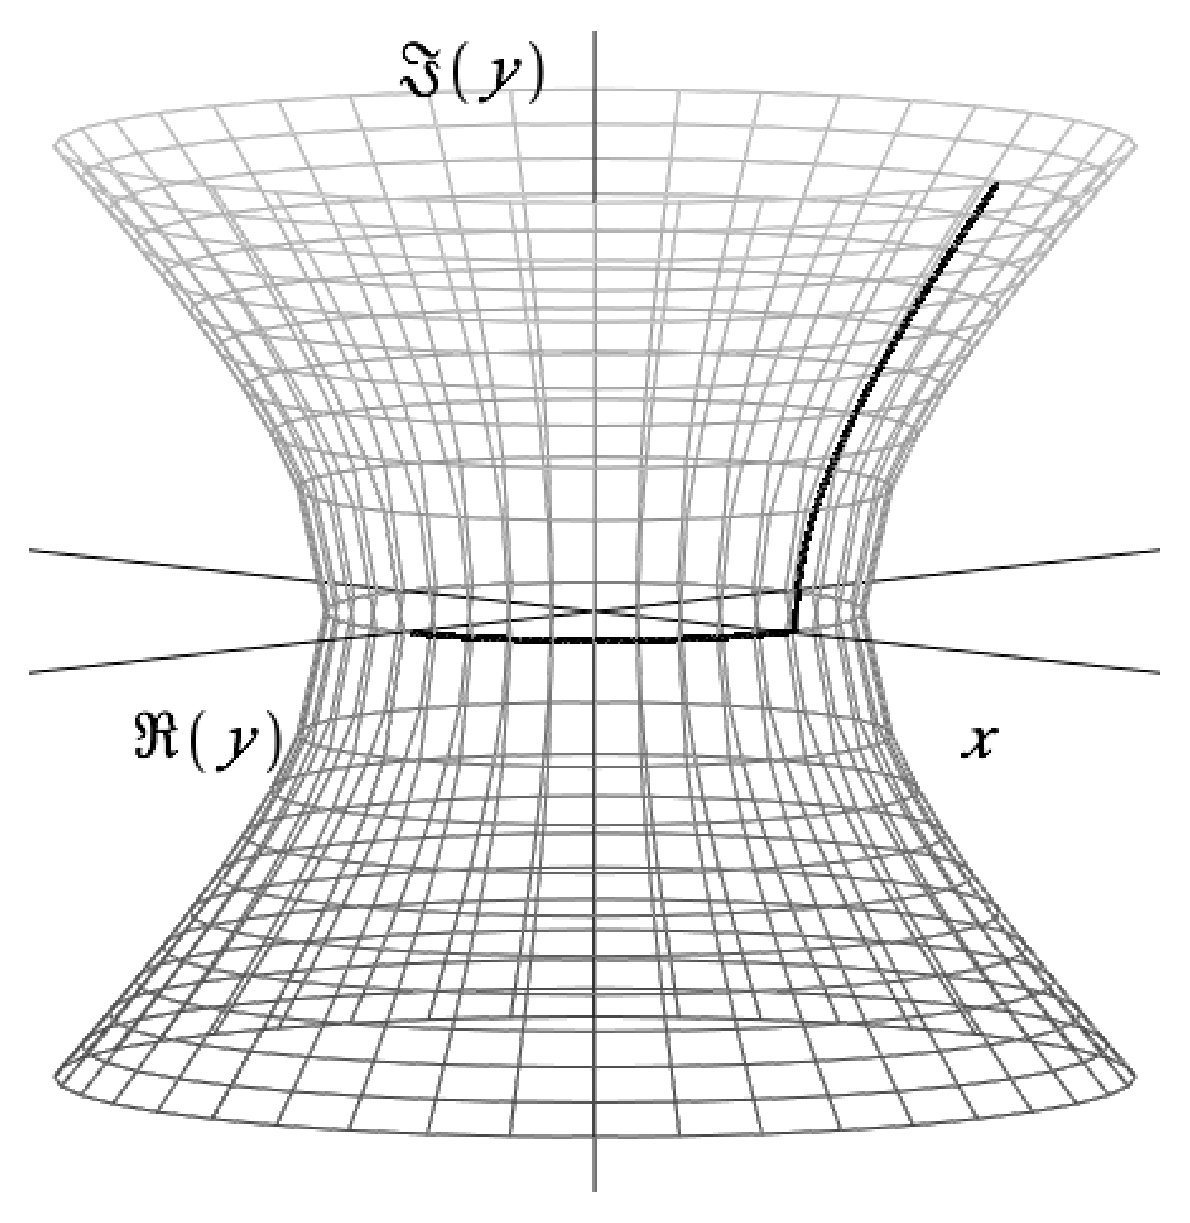
\includegraphics[height=3in]{max_symm_space_graphed.eps}}
\caption[A one-dimensional representation of a positively curved, isotropic surface.]{A one-dimensional analogue of the surface described by Eq.~(\ref{max_symm_space}) for all $r>0$, when $\Lambda>0$, plotted on the two-dimensional hyperboloid of one sheet in $\mathbb{M}^3$.}\label{max_symm_space_graphed}
\end{figure}
We have therefore discovered, through a simple continuous rescaling of the radial coordinate, viz.~Eq.~(\ref{r(t)}), that the geometry to which Eq.~(\ref{max_symm_space}) corresponds most objectively, is not `\textit{either} the closed 4-sphere \textit{or} four-dimensional de~Sitter space, depending on the appropriate range of $r$', but is in fact five-dimensional de~Sitter space---which may be described as a five-dimensional hyperboloid of one sheet, embedded in six-dimensional Minkowski space,---of which Eq.~(\ref{max_symm_space}) gives a particular continuous ($C^0$) four-dimensional slicing, as follows: beginning from any point on the hyperboloid's equator, the line-element extends $90^{\circ}$ along the equator---i.e., along the slice of five-dimensional de~Sitter space in six-dimensional Minkowski space, that describes a closed 4-sphere of radius $\sqrt{3/\Lambda}$ embedded in five-dimensional Euclidean space---to reach $r=\sqrt{3/\Lambda}$, and then rotates $90^{\circ}$ (in either direction), in order to continue along a four-dimensional slice which runs perpendicular to the plane of the equator. The one-dimensional analogue of this surface---the spherical arc, given by the function $(\mathbb{R},\mathbb{C},\{(x,\sqrt{\alpha^2-x^2}):x\in\mathbb{R}>0\})$---is plotted in Fig.~\ref{max_symm_space_graphed}, on the two-dimensional hyperboloid in three-dimensional Minkowski space, $\mathbb{M}^3\equiv\mathbb{R}\times\mathbb{C}$.

This is why $r=\sqrt{3/\Lambda}$ has to be called a coordinate singularity, because it is clearly not meaningful to say that the curvature goes to infinity near that point \cite{Schmidt1971}; rather, this peculiar slicing is the result of our prior attempt to describe an open, positively curved Riemannian manifold, using spherical coordinates that would extend all the way in to the origin, when the geometry does not actually exist within a well-defined limit in the flat embedding space---so the line-element pivots ninety degrees when it reaches that point, and continues on to the completion of $r$. Therefore, when we consider the fact that the closed sphere can really be described as a subspace, of arbitrary constant radius, of any of the three other maximally symmetric spaces, it seems likely that it is only given explicit formulation in our solution, Eq.~(\ref{max_symm_space}), when $\Lambda>0$, because de~Sitter space is a one-sheeted hyperboloid which has a minimum radius; so it seems far more consistent to describe de~Sitter space, rather than the closed sphere, as the positive curvature analogue of the maximally symmetric spaces with zero or negative curvature, and therefore to speculate that this minimum $r$, as well as the Lorentzian signature, should really be intrinsic properties resulting specifically from that positive curvature. It is therefore important to examine in greater detail, the global description of the spaces with complete radial symmetry, in order to find a description that offers an objective explanation of these interesting possibilities. 

In fact, if we refer back to Eqs.~(\ref{Lorentz_sphere1}) -- (\ref{Lorentz_sphere2}), we should note that this particular slicing of Minkowski space actually does objectively describe all three cases; e.g., when $\Lambda<0$, Eq.~(\ref{Lorentz_sphere2}) describes a hyperboloid of two sheets, which, when embedded---i.e., as a \textit{spacelike} hypersurface---in Minkowski space, describes the negative curvature analogue of de~Sitter space, which has four positive-definite eigenvalues. This can be shown explicitly, by replacing Eqs.~(\ref{dS_hyperboloid1}) -- (\ref{dS_hyperboloid2}) with
\begin{equation}
x_0=\sqrt{\frac{3}{|\Lambda|}}\cosh\left(\sqrt{\frac{|\Lambda|}{3}}t\right),\label{AdS_hyperboloid1}
\end{equation}
\begin{equation}
x_i=\sqrt{\frac{3}{|\Lambda|}}\sinh\left(\sqrt{\frac{|\Lambda|}{3}}t\right)z_i,~~~1\leq{i}\leq4,\label{AdS_hyperboloid2}
\end{equation}
so that Eq.~(\ref{Lorentz_sphere1}) becomes instead,
\begin{equation}
ds^2=dt^2+\frac{3}{|\Lambda|}\sinh^2\left(\sqrt{\frac{|\Lambda|}{3}}t\right)d{\Omega_3}^2
\end{equation}
(cf.~Eq.~(\ref{max_symm_round})).

Furthermore, it is significant that if we simply replace $x_0\mapsto{ix_0}$, Eqs.~(\ref{Lorentz_sphere1}) -- (\ref{Lorentz_sphere2}) describe an embedding of the closed sphere of radius $\sqrt{3/\Lambda}$ in $\mathbb{R}^5$. For this reason, it is appropriate to refer to the maximally symmetric hypersurfaces of $\mathbb{M}^5$, which can all be described objectively by Eqs.~(\ref{Lorentz_sphere1}) -- (\ref{Lorentz_sphere2}), also as four-dimensional `spheres' with radius $\alpha\equiv\sqrt{3/\Lambda}$ (see Figure~\ref{Lorentz_sphere}; the formal justification for referring to all of these surfaces as `spheres' will be made yet more explicit in what follows---especially through the analysis leading to Eq.~(\ref{sphere3}), below).

\begin{figure}[t!]
\centerline{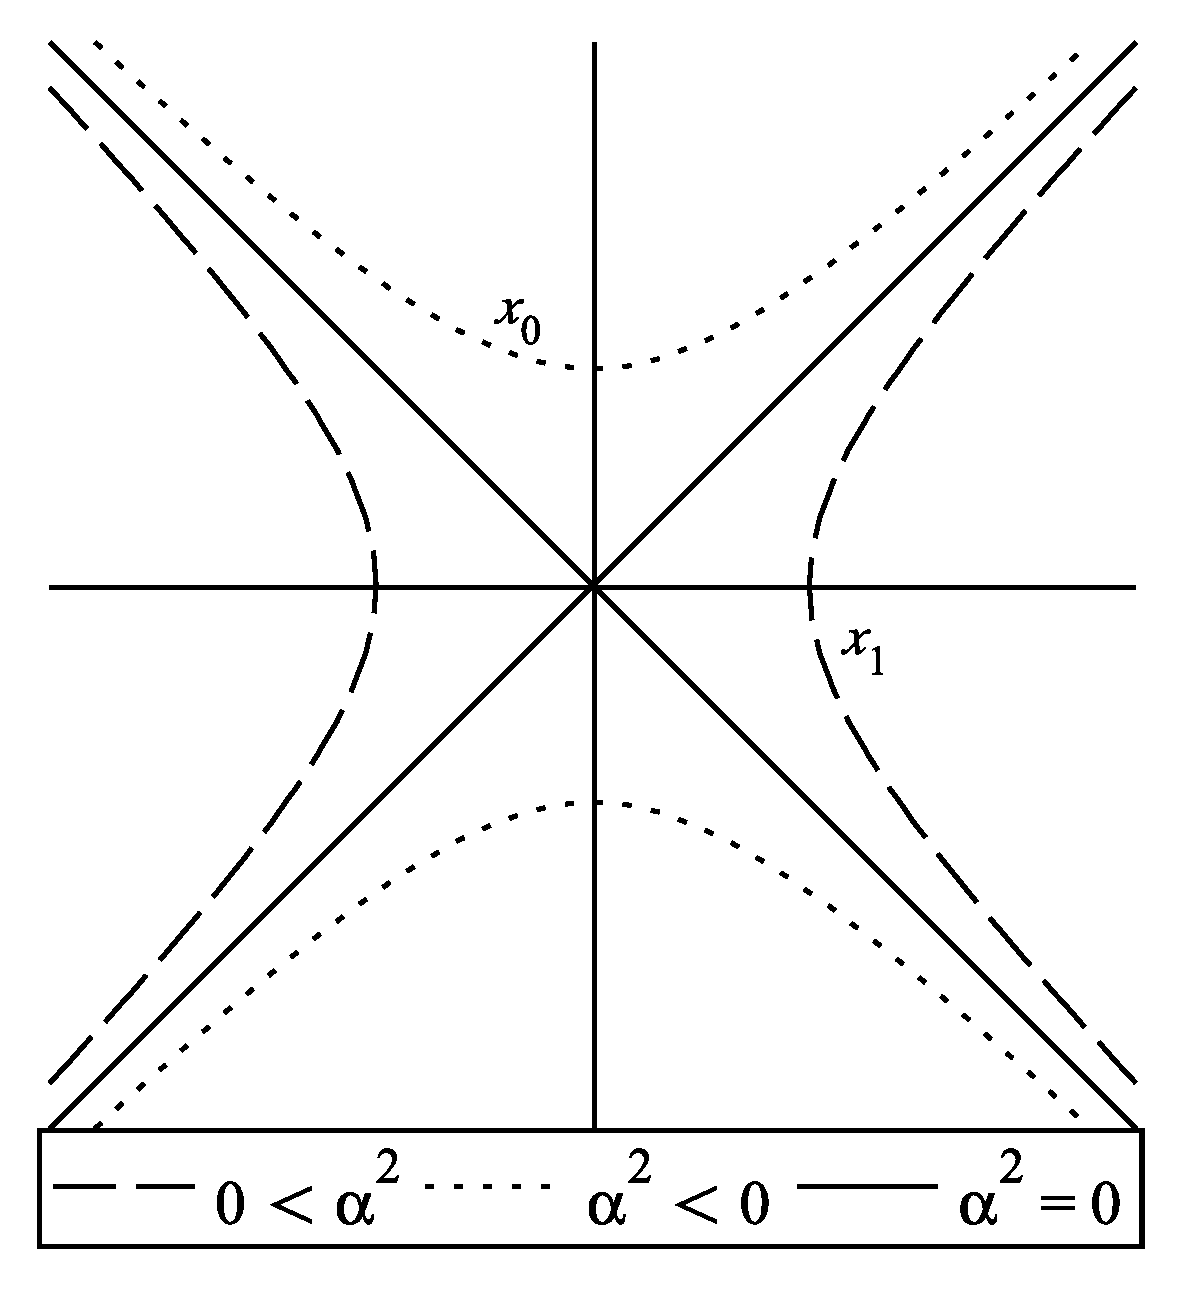
\includegraphics[width=3.26in]{Lorentz_sphere.eps}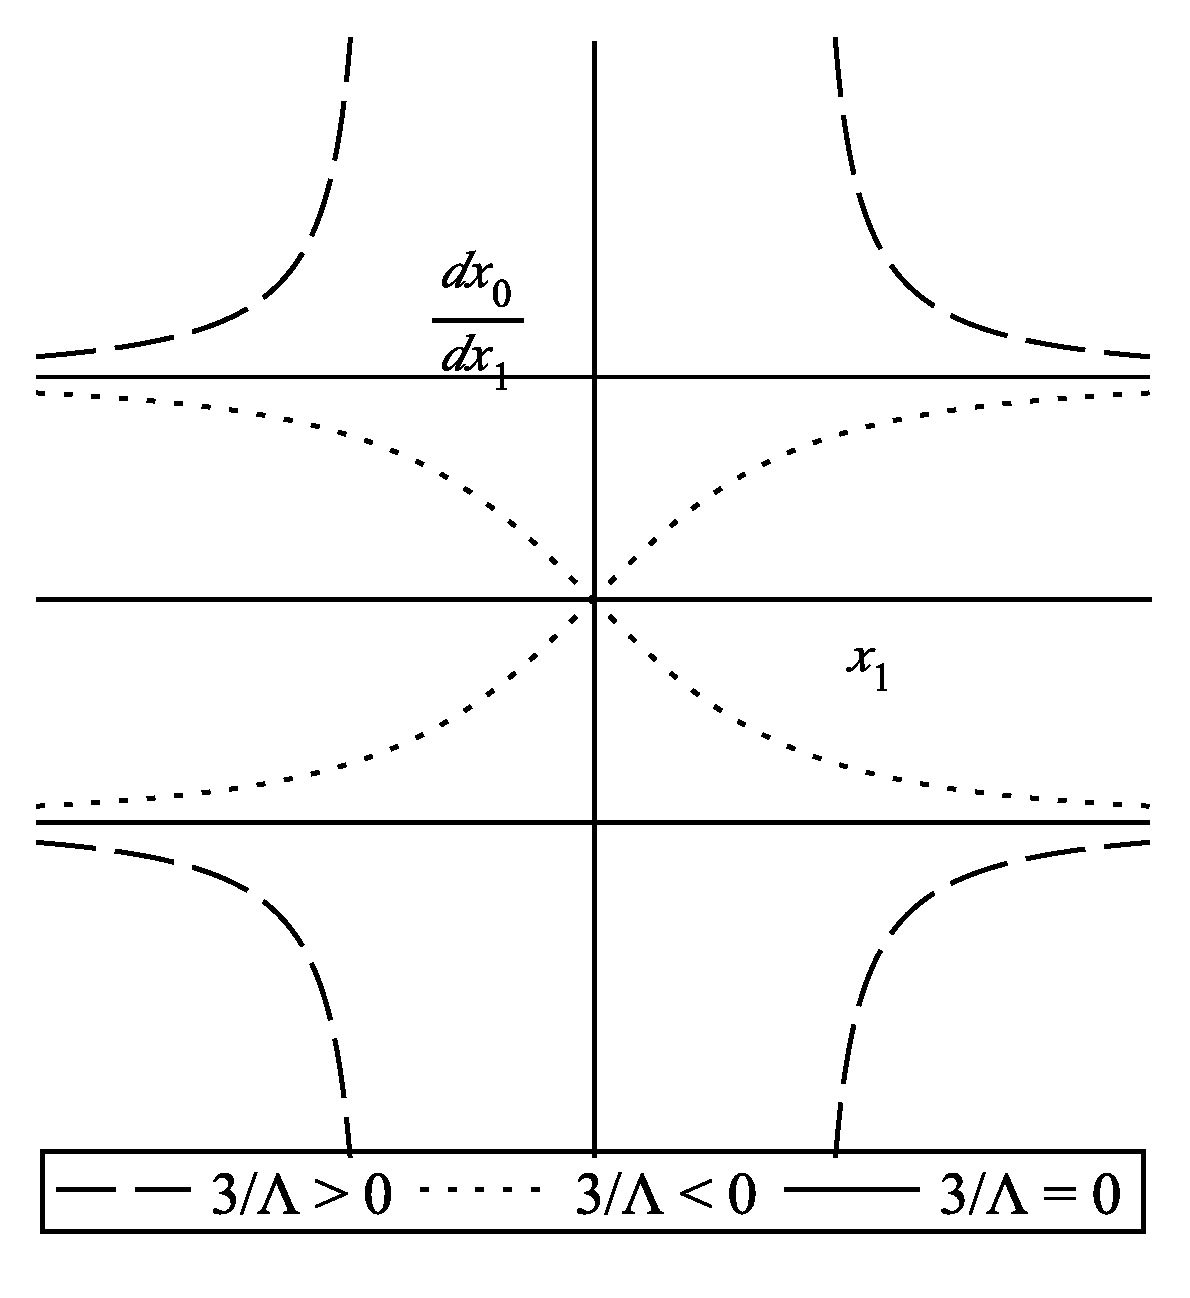
\includegraphics[width=3.26in]{Lorentz_sphere_diff.eps}}
\caption[The sphere in $\mathbb{M}^2$.]{Representations, in $\mathbb{M}^2$, of the one-dimensional spheres with positive, negative, and zero radius, $\alpha$ (left), along with the derivative of each surface with respect to the spatial coordinate, $x_1$ (right). Higher-dimensional spheres are the rotations of these curves about the $x_0$-axis.}\label{Lorentz_sphere}
\end{figure}

It follows at once that geometrically distinct spherical hypersurfaces of $\mathbb{M}^5$ are described when $\alpha^2$ is positive, negative, and zero: sc., when $\alpha^2$ is (i.) positive, the sphere is de~Sitter space---the maximally symmetric timelike hypersurface of $\mathbb{M}^5$ with positive extrinsic curvature, which is bounded according to $\sum_{i=1}^4{x_i}^2=\alpha^2+{x_0}^2>\alpha^2$,---(ii.) negative, the sphere is `Anti-de~Sitter space'---the maximally symmetric spacelike hypersurface with negative extrinsic curvature, which is bounded according to $x_0^2=-\alpha^2+\sum_{i=1}^4{x_i}^2>-\alpha^2$,---and (iii.) zero, the sphere is the null hypersurface defined by the cone, $x_0^2=\sum_{i=1}^4{x_i}^2$, with zero extrinsic curvature---i.e., the zero-radius sphere, with $ds=0$, is a (flat) light cone of the Minkowski space in which it is embedded.

Now, it must be noted that these are all (pseudo-)Riemannian manifolds, which do not need to be described as surfaces embedded in a higher-dimensional space, with extrinsic curvature---although this is useful for visually contrasting the distinct geometries,---but can in fact be described explicitly as four-dimensional Riemannian manifolds with constant \textit{intrinsic} curvature, which all satisfy the relevant field equation,
\begin{equation}
R_{kilj}=\frac{1}{\alpha^2}(g_{kl}g_{ji}-g_{kj}g_{li}),
\end{equation}
and therefore,
\begin{equation}
R_{ij}={R^{k}}_{ikj}=\frac{(n-1)}{\alpha^2}g_{ij};
\end{equation}
so, although the embeddings just described have been useful for forming some intuition about each manifold, and about the differences between them, it is important to note that our analysis here has effectively amounted to an attempt at describing our assumed Void's basic state, if its curvature would be nowhere influenced by the presence of any mass, as a real four-dimensional maximally symmetric manifold.

Some recapitulation should help to clarify this significant point, to which much of our theoretical development has been converging. In \S~\ref{sec_ARP}, we said that if there is actually a four-dimensional Void, then it should always have to obey the same gravitational field law as the Universe does, since the matter in the Universe is supposed to move through It and that law, which amounts to $R_{\mu\nu}\propto{g_{\mu\nu}}$ everywhere the stress-energy vanishes, has apparently held consistently in the Universe throughout Time. And in this section, we've been investigating the solution of this equation that describes a total vacuum which is perfectly isotropic and homogeneous. As our theoretical void goes, we've also assumed that it should subsist in Reality, regardless of any matter it might contain, and we've also assumed, in \S~\ref{sec_ANE}, a principle of Natural Order---that there are basic Truths, or Natural Laws, which hold consistently throughout Physical Reality. In addition to this, we recognise the general principle of relativity theory, which requires the (empirically motivated, rationally inferred, mathematically formulated, and empirically confirmed) basic theoretical laws of physics to be a frame-independent property of Physical Reality. 

But this all comes pretty well in line with an assumption that the void's basic `ground' state should be one of the spherical solutions we've been investigating; i.e., that along with describing the vacuum spacetime geometry outside any massive source that may exist, we take Einstein's equation to be the statement of a basic physical law, that in Reality there subsists, in accordance with the Natural Order we must assume to hold throughout---so that, e.g., an Earthly electron travelling through space, say to the Coma cluster, would not become something else simply as a result of that motion, such as a stereo system pumping \textit{Van Halen} at full blast, but would in fact remain an electron unless something occurred to alter its state of existence through some other demonstrable law of physics,---a four-dimensional Riemannian manifold with intrinsic maximal symmetry, which we call the Void.

But then the problem still remains, that aside from the description of the closed 4-sphere as a real four-dimensional hypersurface of $\mathbb{R}^5$, the rest have just been described by embeddings in an imaginary `Minkowskian' space, $\mathbb{M}^5\equiv\mathbb{C}\times\mathbb{R}^3$. So, let us take a step back once more, while keeping in mind the results of our discussion up to this point, and re-examine the general solution, beginning from the description of a 4-sphere with radius $\alpha$, embedded in flat five-dimensional space, with line-element,
\begin{equation}
ds^2=\sum_{\mu=0}^{4}{dx_{\mu}}^2,\label{R5}
\end{equation}
according to the equation,
\begin{equation}
\sum_{\mu=0}^4{x_{\mu}}^2=\alpha^2.\label{sphere1}
\end{equation}
By solving for $x_0$ (without loss of generality) as a function of the other four coordinates,
\begin{equation}
x_0=\pm\sqrt{\alpha^2-\sum_{i=1}^4{x_i}^2},\label{sphere2}
\end{equation}
this surface can be described equivalently as a four-dimensional manifold with line-element,
\begin{equation}
ds^2=d\mathbf{x}^2+\frac{(\mathbf{x}\cdot{d\mathbf{x}})^2}{\alpha^2-\mathbf{x}^2},\label{sphere3}
\end{equation}
where $\mathbf{x}=(x_1,x_2,x_3,x_4)$ is a real four-dimensional vector in its tangent space.

In fact, Eq.~(\ref{sphere3}), with $-\infty\leq\alpha^2\leq\infty$, can be used to describe all maximally symmetric four-dimensional spaces, so long as appropriate ranges are assumed for the $x_i$s, since it describes the same geometry as Eq.~(\ref{max_symm_space}), in Cartesian coordinates with $\alpha^2=3/\Lambda$ (cf.~Eq.~(13.3.3) in \cite{Weinberg1972}, with $K=\alpha^{-2}$). 

And the significance of $\mathbb{M}^5$ as an embedding space for every case other than the one for which $\alpha^2>0$ and $\alpha^2>\mathbf{x}^2$, should be clear from Eq.~(\ref{sphere2}), since $x_0$ must be purely imaginary otherwise, in which case Eqs.~(\ref{R5}) -- (\ref{sphere1}) can be rewritten according to $x_0\mapsto{ix_0}$, so that $x_{\mu}\in\mathbb{R}~\forall~\mu\in\{0,...,4\}$---but according to the description given by Eq.~(\ref{sphere3}), $x_0$ is not actually a coordinate of the four-dimensional manifold, which is purely real, as the $x_i$s describing the surface are all real, regardless of the value of $\alpha^2$. 

Furthermore, from Eq.~(\ref{sphere3}) it is possible to read off the corresponding elements of the metric tensor,
\begin{equation}
g_{ij}=\frac{1}{\alpha^2-\mathbf{x}^2}\left\{\begin{array}{ll}
\alpha^2-(\mathbf{x}^2-{x_i}^2), & i=j \\ 
x_ix_j, & i\neq{j}
\end{array}\right.,\label{sphere4}
\end{equation}
which always has three positive eigenvalues, along with
\begin{equation}
\lambda=\frac{\alpha^2}{\alpha^2-\mathbf{x}^2},\label{eigenvalue}
\end{equation}
as expected; i.e., when $\alpha^2<0$, $\alpha^2=\pm\infty$ ($\Lambda=0$), or when $\alpha^2>0$ and $\alpha^2>\mathbf{x}^2$, $\lambda>0$; when $\alpha^2=0$, $\lambda=0$; and when $\mathbf{x}^2>\alpha^2>0$, $\lambda<0$.

This proves the anticipated result: that de~Sitter space, with $\mathbf{x}^2>\alpha^2>0$, is the only real Riemannian manifold that has maximal symmetry and intrinsic Lorentzian signature; i.e., it is a Riemannian manifold, with a real coordinate basis, which satisfies the symmetry requirement of our theory, and it is the only one of these with the requisite causal structure. In contrast, when $\lambda>0$, the maximally symmetric spaces with positive-definite metric tensor require an \textit{ad hoc} definition of cosmic time---e.g., which, according to our discussion in \S\S~\ref{sec_OJGKD} -- \ref{sec_ARP}, can be imposed on four-dimensional Euclidean space by setting $x_i=it$ for some arbitrary Cartesian coordinate, $x_i$, in order to impose the pseudo-Lorentzian signature of complex Minkowski space, that is required for the covariant description of spacetime events that occur in a special relativistic universe.

Now, it is an interesting consequence of the fact that de~Sitter space can be described as a Lorentzian slice of Minkowski space, that although this surface has the shape of a curved hyperboloid of one sheet, the null-lines of de~Sitter space must also satisfy $0=-dx_0^2+\sum_{i}dx_i^2$, and therefore must be straight lines on that curved surface in its higher-dimensional flat embedding space. This can be easily checked, e.g., by considering the equation of motion for some particle travelling along a null-line, according to Eq.~(\ref{max_symm_space}):
\begin{equation}
\theta=\pm\int_{r>\sqrt{3/\Lambda}}\frac{dr}{r\sqrt{\frac{\Lambda}{3}r^2-1}}=\mp\arctan\left(\frac{1}{\sqrt{\frac{\Lambda}{3}r^2-1}}\right)+C,\label{null_eom}
\end{equation}
which has been written in the coordinate system for which that motion occurs in only one spatial direction, $\theta$. But note also, that in the flat Minkowski embedding space, the two-dimensional slice of de~Sitter space on which this motion occurs, is the hyperboloid satisfying
\begin{equation}
{x_0}=\pm\sqrt{{x_1}^2+{x_2}^2-\frac{3}{\Lambda}}=\pm\sqrt{r^2-\frac{3}{\Lambda}},
\end{equation}
where cylindrical coordinates, for which $x_1=r\cos\theta$ and $x_2=r\sin\theta$, have been introduced in the second step. Then, considering the lines for which $C=0$ in Eq.~(\ref{null_eom}), we find the expressions for the corresponding null-lines in Cartesian coordinates:
\begin{equation}
x_1=r\cos\theta=\frac{r}{\sqrt{1+\frac{1}{\frac{\Lambda}{3}r^2-1}}}=\sqrt{r^2-\frac{3}{\Lambda}}=\pm{x_0},
\end{equation}
\begin{equation}
x_2=r\sin\theta=\mp\frac{r}{\sqrt{\frac{\Lambda}{3}r^2-1}}\cdot\frac{1}{\sqrt{1+\frac{1}{\frac{\Lambda}{3}r^2-1}}}=\mp\sqrt{\frac{3}{\Lambda}},
\end{equation}
as expected. So, according to Eq.~(\ref{null_eom}), a particle travelling along a null-line will traverse an angle $\pi/2$ on the interval $\sqrt{3/\Lambda}<r<\infty$, although two lines separated by an angle $\pi$ at $r=\sqrt{3/\Lambda}$ will run parallel to each other, through the flat embedding space, and will therefore never meet.

In this analysis, we have indeed found an answer to the unasked question that was at the heart of Einstein's statement, when he said, `The non-divisibility of the four-dimensional continuum of events does not at all, however, involve the equivalence of the space co-ordinates with the time co-ordinate. On the contrary, we must remember that the time co-ordinate is defined physically wholly different from the space co-ordinates' \cite{Einstein1945}; for, rather than imposing this distinction between time and space as an abstract fact, as Einstein had to do because he believed in the relative simultaneous realities that can be described in the spacetime continuum, we now understand that this distinction is related to the requirement of a dynamic cosmic time, which can be formally described either by the \textit{ad hoc} assumption of an absolute motion, which may be explicitly formulated through an imaginary coordinate transformation in one arbitrary direction of four-dimensional space, or it may actually be an intrinsic property of the Void, if its ground state would be four-dimensional de~Sitter space.

And the fact that de~Sitter space is the only maximally symmetric Riemannian manifold that possesses an intrinsic Lorentzian signature, suggests that Eddington was probably correct when he claimed that, `to drop the cosmical constant would knock the bottom out of space' \cite{Eddington1933}, which Chandrasekhar saw fit to denigrate in a centenary lecture held in his memory, when he said, `it is clear that no serious student of relativity is likely to subscribe to [this] view' \cite{Chandrasekhar1983}; for in fact, setting $\Lambda\leq0$ really does knock the relativistic metrical structure out of an underlying maximally symmetric void.

Actually, Eddington had stated his argument for this conclusion in more detail in \cite{Eddington1923}, and it is very useful to refer back to his original reasoning, because, along with being relevant to our current analysis, it also relates back to the problem of the existence of real particles in spacetime, although some of the inferences he makes are obviously different from the ones made here; therefore, we shall consider the argument in his section dealing with the interpretation of Einstein's law of gravitation, in which a brief analysis leads him to a conclusion quite similar to ours---viz., that
\begin{quotation} 
\ldots the radius of curvature in every direction and at every point in empty space has the constant length $\sqrt{3/\Lambda}$.

Conversely if the directed radius of curvature in empty space is homogeneous and isotropic Einstein's law will hold.

The statement that the radius of curvature is a constant length requires more consideration before its full significance is appreciated. Length is not absolute, and the result can only mean \textit{constant relative to the material standards of length} used in all our measurements and in partiular in those measurements which verify $R_{\mu\nu}={\Lambda}g_{\mu\nu}$. In order to make a direct comparison the material unit must be conveyed to the place and pointed in the direction of the length to be measured. It is true that we often use indirect methods avoiding actual transfer or orientation; but the justification of these indirect methods is that they give the same result as a direct comparison, and their validity depends on the truth of the fundamental laws of nature. We are here discussing the most fundamental of these laws, and to admit the validity of the indirect methods of comparison at this stage would land us in a vicious circle. Accordingly the precise statement of our result is that the radius of curvature at any point and in any direction is in constant proportion to the length of a specified material unit placed at the same point and oriented in the same direction.

This becomes more illuminating if we invert the comparison---
\begin{eqnarray}
~~~~\nonumber{\textit{The length of a specified material structure bears a constant ratio to the radi-}}\\
\textit{us of curvature of the world at the place and in the direction in which it lies.~~~~~}\label{Edd_law}
\end{eqnarray}

The law no longer appears to have any reference to the constitution of an empty continuum. It is a law of material structure showing what dimensions a specified collection of molecules must take up in order to adjust itself to equilibrium with surrounding conditions of the world.

The possibility of the existence of an electron in space is a remarkable phenomenon which we do not yet understand. The details of its structure must be determined by some unknown set of equations, which apparently admit of only two discrete solutions, the one giving a negative electron and the other a positive electron or proton. If we solve these equations to find the radius of the electron in any direction, the result must necessarily take the form
\begin{itemize}
\item[~]radius of electron in given direction = numerical constant $\times$ some function of the conditions in space into which the electron was inserted.
\end{itemize}
And since the quantity on the left is a directed length, the quantity on the right must be a directed length. We have just found one directed length characteristic of the empty space in which the electron was introduced, viz.~the radius of the spherical curvature of a corresponding section of the world. Presumably by going to the third or fourth derivatives of the $g_{\mu\nu}$ other independent directed lengths could be constructed; but that seems to involve an unlikely complication. There is strong ground then for anticipating that the solution of the unknown equations will be
\begin{itemize}
\item[~]radius of electron in any direction = numerical constant $\times$ radius of curvature of space-time in that direction. 
\end{itemize}
This leads at once to the law (\ref{Edd_law}).

As with the electron, so with the atom and aggregations of atoms forming the practical units of material structure. Thus we see that Einstein's law of gravitation is the almost inevitable outcome of the use of material measuring-appliances for surveying the world, whatever may be the actual laws under which material structures are adjusted in equilibrium with the empty space around them.

Imagine first a world in which the curvature, referred to some chosen (non-material) standard of measurement, was not isotropic. An electron inserted in this would need to have the same anisotropy in order that it might obey the same detailed conditions of equilibrium as a symmetrical electron in an isotropic world. The same anisotropy persists in any material structure formed of these electrons. Finally when we \textit{measure} the world, i.e.~make comparisons with material structures, the anisotropy occurs on both sides of the comparison and is eliminated. Einstein's law of gravitation expresses the result of this elimination. The symmetry and homogeneity expressed by Einstein's law is not a property of the external world, but a property of the operation of measurement.

From this point of view it is inevitable that the constant $\Lambda$ cannot be zero; so that empty space has a finite radius of curvature relative to familiar standards.\footnote{He implicitly assumes the fact that no one should consider it a real physical possibility that the radius of curvature could actually be imaginary.} An electron could never decide how large it ought to be unless there existed some length independent of itself for it to compare itself with.

It will be noticed that our rectangular coordinates $(x_1, x_2, x_3, x_4)$ in this and the previous section approximate to Euclidean, not Galilean, coordinates. Consequently $x_4$ is imaginary time, and $G_{(4)}$ is not in any real direction in this world.\footnote{The errors made in this paragraph and the next one have to do with some of the points that have been discussed in our analysis so far, according to which they should be mentally corrected by the reader---for it remains relevant to us to see where Eddington was going with this.} There is no radius of curvature in a real timelike direction. This does not mean that our discussion is limited to three dimensions; it includes all directions in the four-dimensional world outside the light-cone, and applies to the space-dimensions of material structures moving with any speed up to the speed of light. The real quadric of curvature terminates at the light-cone, and the mathematical continuation of it lies not inside the cone but in directions of imaginary time which do not concern us.

By consideration of extension in timelike directions we obtain a confirmation of these views, which is, I think, not entirely fantastic. We have said that an electron would not know how large it ought to be unless there existed independent lengths in space for it to measure itself against. Similarly it would not know how long it ought to exist unless there existed a length in time for it to measure itslef against. But there is no radius of curvature in a time-like direction; so the electron does \textit{not} know how long it ought to exist. Therefore it just goes on existing indefinitely.

The alternative laws of gravitation discussed in \S~62 [Alternative energy-tensors] would be obtained if the radius of the unit of material structure adjusted itself as a definite fraction not of the radius of curvature, but of other directed lengths (of a more complex origin) characteristic of empty space-time.

In \S~56 [Dynamics of a particle] it was necessary to postulate that the gravitational field due to an ultimate particle of matter has symmetrical properties. This has now been justified. We have introduced a new and far-reaching principle into the relativity theory, viz.~that symmetry itself can only be relative; and the particle, which so far as mechanics is concerned is to be identified with its gravitational field, is the standard of symmetry. We reach the same result if we attempt to define symmetry by the propagation of light, so that the cone $ds=0$ is taken as the standard of symmetry. It is clear that if the locus $ds=0$ has complete symmetry about an axis (taken as the axis of $t$) $ds^2$ must be expressible by [the most general possible solution that is spherically symmetric in space, symmetric as regards past and future time, and is static,
\begin{equation}
ds^2=-U(r)dr^2-V(r)(r^2d\theta^2+r^2\sin^2\theta{d\phi}^2)+W(r)dt^2,
\end{equation}
where $U$, $V$, $W$ are arbitrary functions of $r$.]
\end{quotation}

Our analysis has led to many conclusions which are somewhat similar to those Eddington has stated in this exerpt: viz., above, we've found that in order for the void itself, prior to the existence of mass, to intrinsically possess the Lorentzian signature that is required for general covariance, and for it to intrinsically act as a consistent measuring stick throughout space \textit{and} time, relative to which all measurements could be objectively made, the empty void should be the de~Sitter sphere, with $\Lambda>0$. Furthermore, we've seen that photon geodesics are somehow important in the dynamical theory; therefore, it could be possible to use them as the standard of symmetry, in the way Eddington suggests. However, in contrast to Eddington's argument, our results suggest that there can be no `ultimate particle of matter', and that the time-dimension of de~Sitter space is actually as real as the dimensions of space; therefore, his speculation, that `the electron just goes on existing indefinitely', which he based on his own understanding of both of these points, cannot be true. Instead, we've said above, that the existence of physical mass might be a property of a particle's motion relative to photon geodesics; viz., that any energetic particle which moves with respect to photon geodesics might have a measureable mass when it is considered to be at rest in spacetime, as a result of that motion. 

When the results of this section are considered objectively, the possibility emerges, that if there is really no such thing as a particle with intrinsic mass, but that mass should really be a property of motion through the void, as we've found reason to suspect, then the truth may in fact be that the void does not actually dynamically warp in the presence of massive particles, but that it might actually just be de~Sitter space, with the universe moving uniformly through it, and with the physical properties of matter, such as the apparent warping of spacetime around massive objects, actually corresponding to the perception of things therein, i.e.~according to the principle of equivalence. 

Then, the most immediate points to consider, are how the universe should actually evolve through de~Sitter space, and how the paths of various particles are to be described in relation to that.

According to our analysis of de~Sitter space, the most obvious possibility is that the universe could be the expanding 3-sphere that moves uniformly along $r$, in Eq.~(\ref{max_symm_space}), beginning from a finite size at $r=\sqrt{3/\Lambda}$; or, equivalently, which evolves uniformly from a finite-sized beginning, at $t=0$ in
\begin{equation}
ds^2=-dt^2+\frac{3}{\Lambda}\cosh^2\left(\sqrt{\frac{\Lambda}{3}}t\right){d\Omega_3}^2;\label{dS_comoving_univ}
\end{equation} 
and although this is indeed the description that will be given eventually, it is illustrative to first consider some other well-known solutions. 

First, let us consider Eddington's statical frame, Eq.~(\ref{deSitter_statical}),
\begin{equation}
ds^2=-\left(1-\frac{\Lambda}{3}r_{\mathrm{Edd}}^2\right)dt_{\mathrm{Edd}}^2+\frac{dr_{\mathrm{Edd}}^2}{1-\frac{\Lambda}{3}r_{\mathrm{Edd}}^2}+r_{\mathrm{Edd}}^2d\Omega^2,\label{dS_statical}
\end{equation}
which is found from Eqs.~(\ref{Lorentz_sphere1}) -- (\ref{Lorentz_sphere2}), by writing 
\begin{equation}
x_0=\sqrt{\frac{3}{\Lambda}-r_{\mathrm{Edd}}^2}\sinh\left(\sqrt{\frac{\Lambda}{3}}t_{\mathrm{Edd}}\right),\label{dS_statical1}
\end{equation}
\begin{equation}
x_1=\sqrt{\frac{3}{\Lambda}-r_{\mathrm{Edd}}^2}\cosh\left(\sqrt{\frac{\Lambda}{3}}t_{\mathrm{Edd}}\right),\label{dS_statical2}
\end{equation}
\begin{equation}
x_i=r_{\mathrm{Edd}}z_i,~~~2\leq{i}\leq4,\label{dS_statical3}
\end{equation}
where the $z_i$s are defined as above \cite{deSitter2012}. By using Eqs.~(\ref{dS_statical1}) -- (\ref{dS_statical3}), one-dimensional radial slices at constant values of $t_{\mathrm{Edd}}$, as well as the $t_{\mathrm{Edd}}$-evolution at various constant values of $r_{\mathrm{Edd}}$, can be plotted on a two-dimensional slice of the de~Sitter sphere (see Fig.~\ref{fig: dS_statical}).
\begin{figure}[t!]
\centerline{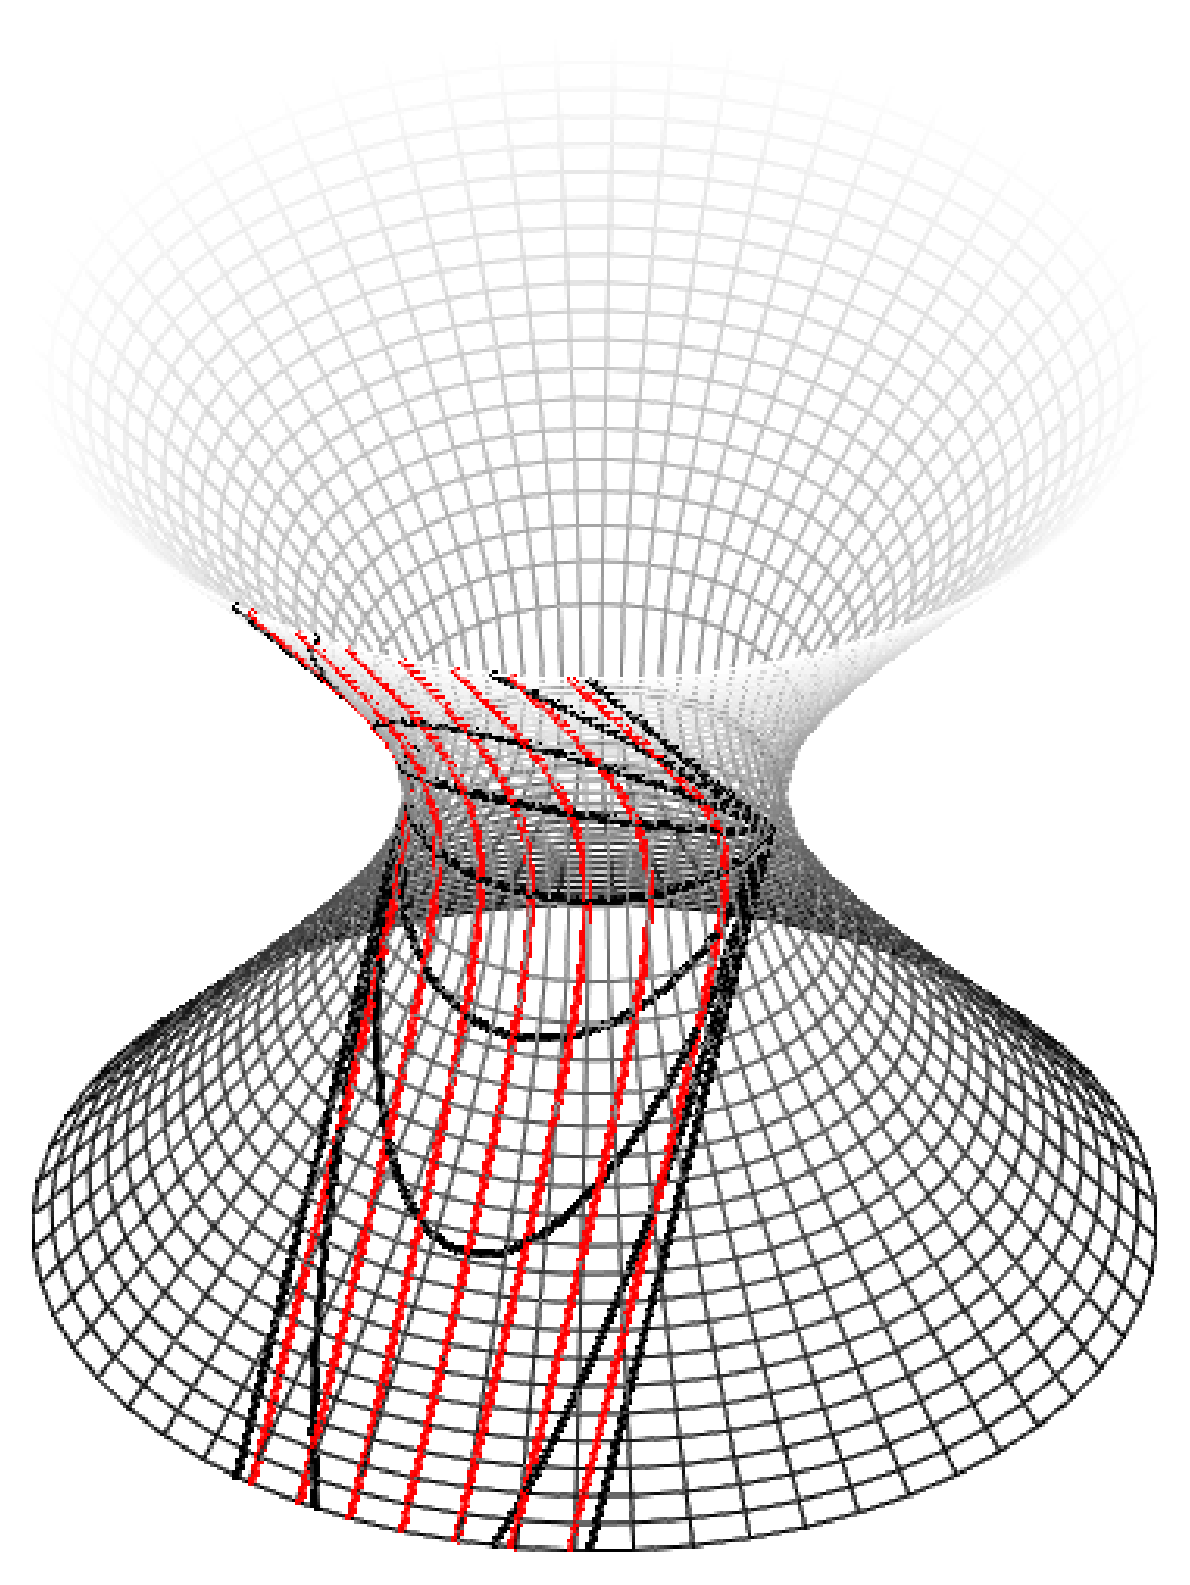
\includegraphics[height=3.75in]{dS_static1.eps}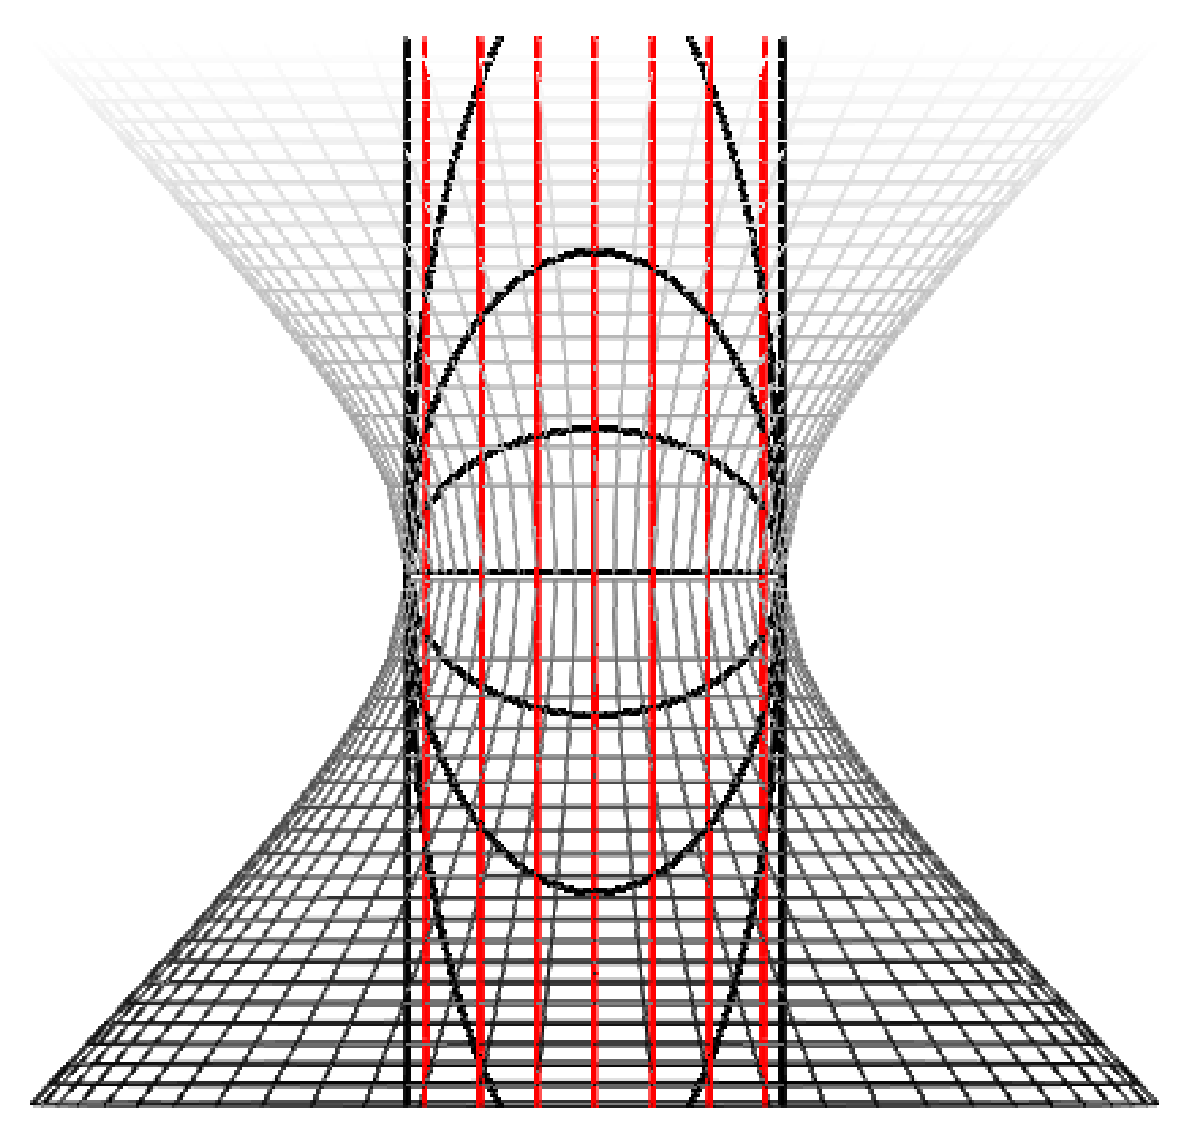
\includegraphics[height=3.5in]{dS_static2.eps}}
\caption[Eddington's statical coordination of de~Sitter space, drawn on the de~Sitter 2-sphere in $\mathbb{M}^3$.]{Slices of constant $t_{\mathrm{Edd}}$, for all possible real values of the radial coordinate, in Eddington's statical coordination of de~Sitter space (black lines), along with (non-geodesic) world-lines of constant $r_{\mathrm{Edd}}$ (red lines), drawn on the de~Sitter 2-sphere in $\mathbb{M}^3$.}\label{fig: dS_statical}
\end{figure}

This form of the metric describes a region of de~Sitter space, symmetric about $t_{\mathrm{Edd}}=0$, that can be described as `the set of locally flat spacelike hypersurfaces that would be perceived, in the frame of a particle at rest at $r_{\mathrm{Edd}}=0$, and travelling from $t_{\mathrm{Edd}}=-\infty$ to $t_{\mathrm{Edd}}=+\infty$, as being globally statical, and extending out to an observational horizon at $r_{\mathrm{Edd}}=\sqrt{3/\Lambda}$.' The prior assumption that is made, is the standard requirement that the paths of photons should be null-lines of the metric space. 

For the central particle, which begins its existence at $t_{\mathrm{Edd}}=-\infty$ ($x_0=-\infty$), it then turns out that the `universe' at that time is also such a null-line, which extends to the horizon at $r_{\mathrm{Edd}}^2=3/\Lambda$ ($x_0=0$);\footnote{Note that the `universe' represented by slices of constant time in Eq.~(\ref{dS_statical}), is only half as large as the slices depicted on the hyperboloid in Fig.~\ref{fig: dS_statical} if it is assumed that $r_{\mathrm{Edd}}\geq0$; i.e., because Fig.~\ref{fig: dS_statical} depicts the central particle's `surroundings' on the part of the de~Sitter sphere that is covered by the coordinate system of Eq.~(\ref{dS_statical}), for $-\sqrt{3/\Lambda}\leq{r_{\mathrm{Edd}}}\leq\sqrt{3/\Lambda}$.} and the event there---or, rather, an event infinitesimally closer than that point---is the one that the central particle would observe at $t_{\mathrm{Edd}}=+\infty$, if a photon were emitted there in the appropriate direction (cf.~our derivation of Schwarzschild spacetime in \S~\ref{sec_ARP}).

Now, it should really be obvious from Fig.~\ref{fig: dS_statical}, that the slices of constant $t_{\mathrm{Edd}}$ in Eq.~(\ref{dS_statical}) cannot be descriptions of a dynamic universe at different values of cosmic time, because  these slices are not comoving; i.e., because, according to Eqs.~(\ref{dS_statical1}) -- (\ref{dS_statical3}), the points in space at larger and larger values of $r_{\mathrm{Edd}}$, out to the singularity at $r_{\mathrm{Edd}}=\sqrt{3/\Lambda}$, must travel through $x_0$ more and more quickly until the universe reaches $x_0=0$, and at slower and slower rates beyond that, up to the universal limit, $r_{\mathrm{Edd}}=\sqrt{3/\Lambda}$, which reaches $x_0=0$ in no $t_{\mathrm{Edd}}$, and remains there forever.

In fact, it should also be clear from Fig.~\ref{fig: dS_statical}, or from the transformation, Eqs.~(\ref{dS_statical1}) -- (\ref{dS_statical2}), that if such a \textit{dynamic} universe could possibly be, with its variable cosmic time depending on spatial location defined in order to maintain causal coherence along synchronous slices, it would \textit{actually} be bounded at this singularity; i.e., that it is not actually correct to say that $r_{\mathrm{Edd}}$ becomes timelike and $t_{\mathrm{Edd}}$ becomes spacelike at the `horizon' of Eq.~(\ref{dS_statical}), as we commonly used to say, based partly on the change in the metric signature, as well as the fact that the curvature does not really go to infinity there---i.e., it's really just another point of maximally symmetric de~Sitter space,---but mostly because spacetime was \textit{really} thought to be described, by relativity theory, as a four-dimensional continuum of events, something like all of de~Sitter space, on which any line-element was merely thought to represent some perception of existence in which the coordinates themselves have no metrical significance.

So, we say that Eddington's coordinates really can't describe a universe in de~Sitter space, as a causally coherent set of worldlines, because this slicing of maximally symmetric space is arbitrarily centred about one coordinate, with rates of timelike evolution corresponding to that arbitrary centre, and with a real spatial boundary that is required for essentially the same reasons. But the situation really only gets marginally better if we try to use the Lema\^{i}tre-Robertson slicing to define the universe; for although this universe is actually comoving, and there is no longer a spatial boundary to it, it is defined by the same arbitrarily special central geodesic as Eddington's, and the causal coherence of its comoving geodesics is a gross misrepresentation of the intrinsic structure of de~Sitter space.

The metric (cf.~Eq.~(\ref{deSitter_comoving})),
\begin{equation}
ds^2=-dt_{\mathrm{LR}}^2+e^{2\sqrt{\frac{\Lambda}{3}}\,t_{\mathrm{LR}}}dy^2,\label{dS_LR}
\end{equation}
is found from Eqs.~(\ref{Lorentz_sphere1}) -- (\ref{Lorentz_sphere2}), by writing, 
\begin{equation}
x_0=\sqrt{\frac{3}{\Lambda}}\sinh\left(\sqrt{\frac{\Lambda}{3}}\,t_{\mathrm{LR}}\right)+\sqrt{\frac{\Lambda}{3}}\frac{r_{\mathrm{LR}}^2}{2}e^{\sqrt{\frac{\Lambda}{3}}\,t_{\mathrm{LR}}},\label{dS_LR1}
\end{equation}
\begin{equation}
x_1=\sqrt{\frac{3}{\Lambda}}\cosh\left(\sqrt{\frac{\Lambda}{3}}\,t_{\mathrm{LR}}\right)-\sqrt{\frac{\Lambda}{3}}\frac{r_{\mathrm{LR}}^2}{2}e^{\sqrt{\frac{\Lambda}{3}}\,t_{\mathrm{LR}}},\label{dS_LR2}
\end{equation}
\begin{equation}
x_i=e^{\sqrt{\frac{\Lambda}{3}}\,t_{\mathrm{LR}}}y_i,~~~2\leq{i}\leq4,\label{dS_LR3}
\end{equation}
where $r_{\mathrm{LR}}^2=\sum_{i}y_i^2$ and $dy^2=\sum_{i}dy_i^2$ \cite{deSitter2012}; and, as before, Eqs.~(\ref{dS_LR1}) -- (\ref{dS_LR3}) have been used to plot the one-dimensional radial slices of this coordinate system, at various times, as well as the time-evolution of a few points in space, for both positive and negative values of $r_{LR}$ (see Fig.~\ref{fig: dS_LR}).
\begin{figure}[t!]
\centerline{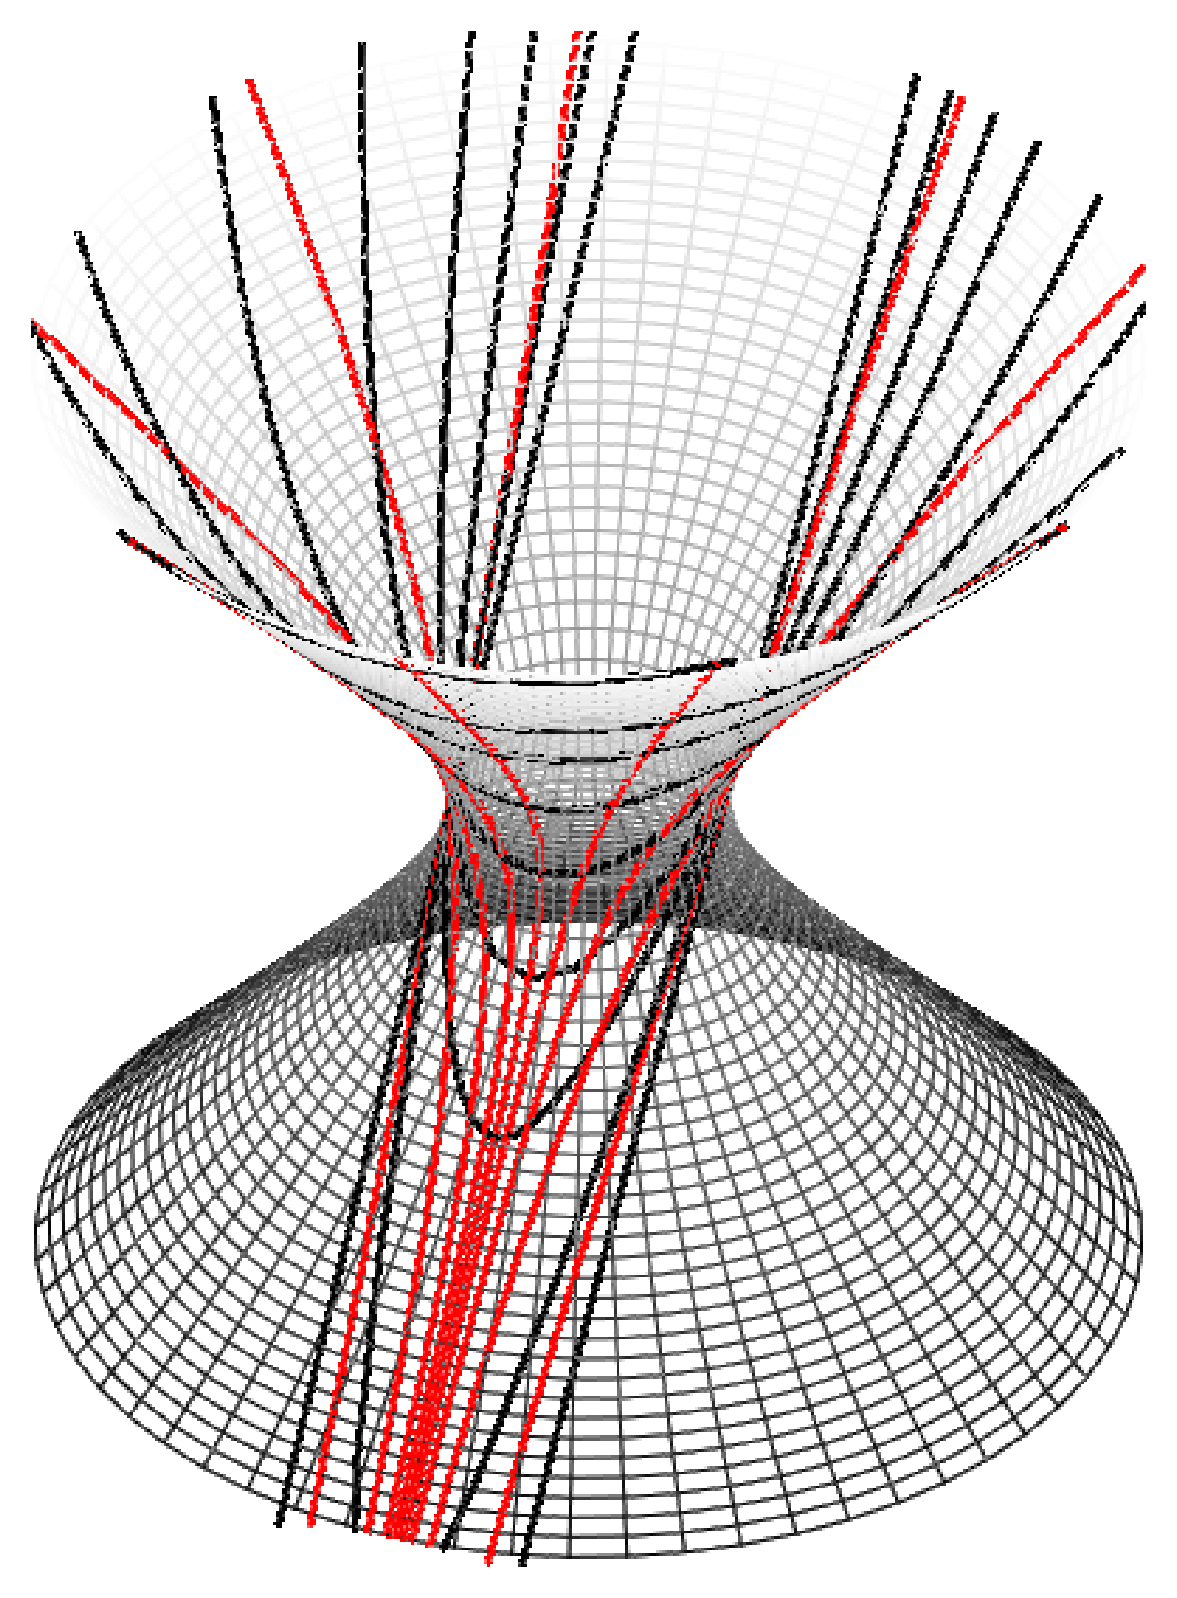
\includegraphics[height=3.75in]{dS_LR1.eps}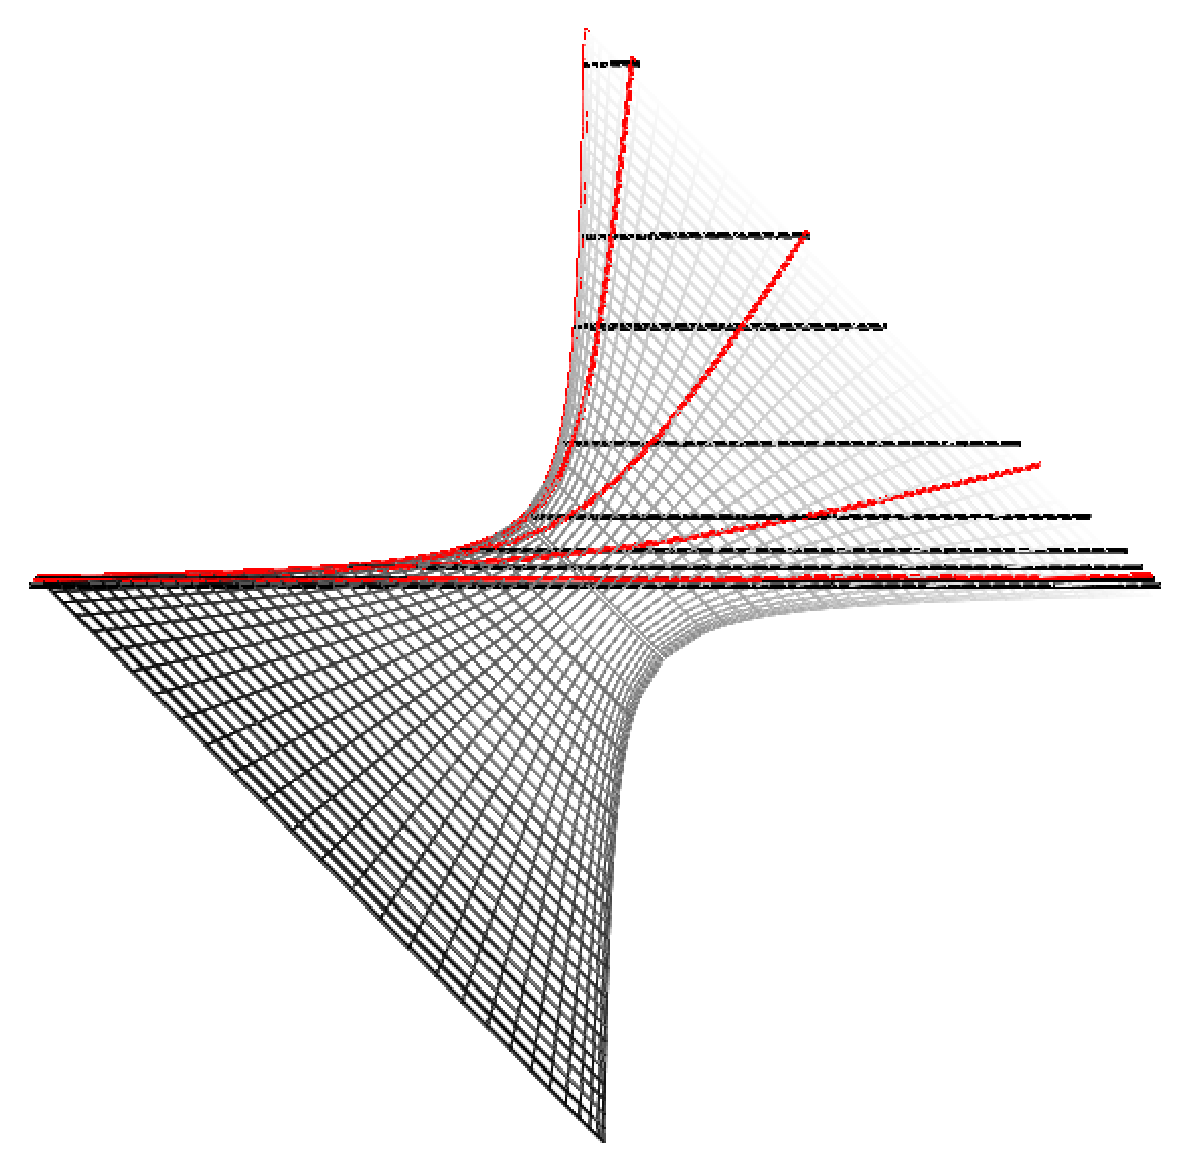
\includegraphics[height=3.75in]{dS_LR2.eps}}
\caption[The Lema\^{i}tre-Robertson coordination of de~Sitter space, drawn on the de~Sitter 2-sphere in $\mathbb{M}^3$.]{Slices of constant time in the Lema\^{i}tre-Robertson coordination of de~Sitter space (black lines), along with comoving geodesic world-lines (red lines), drawn on the de~Sitter 2-sphere in $\mathbb{M}^3$.}\label{fig: dS_LR}
\end{figure}

The fact that the dynamic universe defined by this coordinate system is comoving, is evident from Fig.~\ref{fig: dS_LR}, although this is also immediately obvious from the metric, Eq.~(\ref{dS_LR}), which satisfies the requirement, that $g_{t_{\mathrm{LR}}t_{\mathrm{LR}}}=-1$, along with the requirement that constant spatial coordinates should be geodesics---i.e., that $\partial{g_{it_{\mathrm{LR}}}}/\partial{t_{\mathrm{LR}}}=0$ \cite{Weinberg1972}.

This is the universe that was first described by Weyl.\footnote{It is fair to say that the papers by Lema\^{i}tre \cite{Lemaitre1925b} and Robertson \cite{Robertson1928} were to Weyl's analysis \cite{Weyl1923a,Weyl1923,Weyl2009,Weyl1924,Weyl1930} (see also \cite{Ehlers2009}; a diagram similar to Fig.~\ref{fig: dS_LR} is drawn in \cite{Weyl1924}), as Martin Kruskal's \cite{Kruskal1960} and George Szekeres' \cite{Szekeres1960,Szekeres2002b} were to John Synge's \cite{Synge1950}.} In contrast to Eddington's coordinates, points in space represent particles in free-fall, and although different comoving geodesics move through $x_0$ at different rates, as in Eddington's system, the universe itself progresses uniformly in the $x_0$-direction, though tilted $45^{\circ}$ from that axis, according to Eqs.~(\ref{dS_LR1}) -- (\ref{dS_LR3}). It is bounded by a null-line that pinches off all geodesics to a singular common origin at $x_0=-\infty$, even though the universe, at all cosmic times thereafter, has infinite extent. In fact, it is possible to see clearly how it can be, that this universe, which is infinite in extent, also begins from a single point in de~Sitter space: for although the entire bundle of geodesics emerges from a common origin at $t_{\mathrm{LR}}=-\infty=x_0$---where the spacetime metric is indeed singular,---for all $t_{\mathrm{LR}}>-\infty$ there is always a comoving geodesic connecting this point with another one at arbitrarily large $x_0$, or any $r_{\mathrm{LR}}$, according to Eqs.~(\ref{dS_LR1}) -- (\ref{dS_LR3}), as illustrated in Fig.~\ref{fig: dS_LR}.

However, there is still a cosmological horizon in this universe: i.e., because no information can ever come to an observer at $r_{\mathrm{LR}}=0$ from beyond its backwards light-cone at infinite $t_{\mathrm{LR}}$, the corresponding null-line describes that observer's cosmological horizon. Now, the interesting thing about this, is that because the comoving universe is tilted $45^{\circ}$ from the $x_0$-axis, particles at rest in the universe, travelling along comoving timelike geodesics, should actually be continuously streaming across that horizon for all $t_{\mathrm{LR}}$, though they can only begin to do so after having travelled an infinite distance in the $x_0$-direction. It is tempting to confuse this cosmological horizon---which the central particle would itself inevitably cross, if it would ever take any arbitrarily small step in the $r_{\mathrm{LR}}$-direction---with the singularity at $r_{\mathrm{Edd}}=\sqrt{3/\Lambda}$ in Eddington's coordinate system, and call that a `removable coordinate singularity'; however, although it is true that $r_{\mathrm{Edd}}=\sqrt{3/\Lambda}$ is a singularity only of that ill-defined system, the same point of de~Sitter space is not actually in the Lema\^{i}tre-Robertson universe, for any $t_{\mathrm{LR}}>-\infty$. 

So, the observational horizon, which is actually the same as `space at infinite time' in Eddington's spacetime---i.e., the slice, $t_{\mathrm{Edd}}=+\infty$, of Eq.~(\ref{dS_statical}), which is always perpendicular to the comoving slices, $t_{\mathrm{LR}}=const.$, of Eq.~(\ref{dS_LR}),---has no more significance in the Lema\^{i}tre-Robertson universe than that it is the horizon of the observer who remains at $r_{\mathrm{LR}}=0$; and the fact that other particles would cross that horizon in finite cosmic time, although they would remain visible for all time to that observer, if they would have shone a light in that direction until they crossed the horizon, is ultimately due to the orientation of the evolving universe in de~Sitter space. Even so, this is an interesting point, about which more will be said shortly; however, it is more prudent to first note---what is surely the most astonishing aspect of the Lema\^{i}tre-Robertson universe---that although the dynamic universe, defined by Eqs.~(\ref{dS_LR1}) -- (\ref{dS_LR3}), is \textit{not} actually homogeneous, it would appear so to all comoving observers.

For it is true, according to Eq.~(\ref{dS_LR}), that with photons travelling along null-geodesics, the comoving geodesics of this universe would appear to an observer at $r_{\mathrm{LR}}=0$ as if they actually originated from flat, exponentially expanding space---and so they must also appear the same to all other comoving observers, according to the \textit{spacetime} line-element, even though the actual dynamic universe, at any particular value of cosmic time, is an inhomogeneous slice of de~Sitter space, given by Eqs.~(\ref{dS_LR1}) -- (\ref{dS_LR3}); i.e., although the pre-defined real present is not actually homogeneous (consider, e.g., any slice of constant $t_{\mathrm{LR}}$ in Fig.~\ref{fig: dS_LR}), spatial slices of the four-dimensional spacetime continuum of ideal events, at all values of comoving time in the cosmic rest-frame that is used to describe them, actually are. 

But it is also true, that this particular definition of cosmic time---which requires different comoving geodesics to travel through the de~Sitter sphere with varying rates depending on their distance from $r_{\mathrm{LR}}=0$,\footnote{As defined by Eqs.~(\ref{dS_LR1}) -- (\ref{dS_LR3}), comoving world-lines at larger $r_{\mathrm{LR}}$ traverse greater distances in $x_0$ in equal amounts of cosmic time, as graphed Fig.~\ref{fig: dS_LR}. In other words, the dynamic universe itself, like the Eddington universe, is not fundamentally torsionless, as it is not defined by the trivial tangent bundle of the underlying de~Sitter sphere. Of course, the spacetime still has a Levi-Civita connection because it takes place on the de~Sitter sphere; but the universe itself does not fundamentally coorespond to that connection.} so that they would remain in causally coherent, universal connection,---makes poor use of the natural causal structure of de~Sitter space that was supposed to be significant in our theory: for if we would actually consider such an arbitrarily situated universe to be plausible, it would surely not be any more reasonable a model than another universe, defined on some other Riemannian manifold by introducing its cosmic time in some other, equally arbitrary way, such as an imaginary coordinate transformation.

Furthermore, the actual inhomogeneity of the universe cannot be ignored, despite appearances; i.e., despite the fact that the spatial slices of the metric in Lema\^{i}tre-Robertson coordinates \textit{are} homogeneous for all $t_{\mathrm{LR}}$. For our stated purpose, in continuing the above investigation of maximally symmetric spaces, was that we had wanted to describe the universe as actually being homogeneous at all times, so that every place in the universe would actually be the same as every other place always. We derived our theory based on this assumption, and found that de~Sitter space was the only maximally symmetric Riemannian manifold with real Lorentzian signature---i.e., the only one that intrinsically possesses those null lines which are so important in relativity theory. But this underlying homogeneity is abandoned with any slicing of the de~Sitter sphere that is not actually homogeneous for all times.

With this in mind, we should consider again the fact that comoving geodesics actually do continually cross the horizon of the observer at $r_{\mathrm{LR}}=0$---in fact, that they similarly continually cross the cosmological horizons of all comoving observers in the Lema\^{i}tre-Robertson universe---by making the obvious comparison to the Schwarzschild horizon: for this is actually closely related to the theory of black holes, which was discussed at the end of \S~\ref{sec_ARP}, since a similar description comes from defining a \textit{Finkelstein universe}, as the universe with cosmic time actually given by the advanced time parameter in the Eddington-Finkelstein coordinate system, so that the Schwarzschild horizon has a similar description as the cosmological horizon in the Lema\^{i}tre-Robertson universe, with the main exception being that it is the same horizon for all external observers.

But in \S~\ref{sec_ARP}, it was observed that the Schwarzschild time should actually be the local measure of cosmic time at $r_{\mathrm{Sch}}=\infty$ in the pseudo-Riemannian spacetime solution that describes the evolution of a spherically symmetric star, and that the Schwarzschild metric should be completely meaningless for $r_{\mathrm{Sch}}<2m$, where $r_{\mathrm{Sch}}$ is not simply `timelike', but actually does not exist, just as $r_{\mathrm{Edd}}>\sqrt{3/\Lambda}$ does not exist, and the change in metric signature there is due to the fact that this spatial coordinate becomes imaginary in a metrically insignificant way. Actually, it is not that there is anything theoretically \textit{wrong} with the Finkelstein universe, in the sense of a superficial dynamical interpretation of relativistic spacetime, aside from geodesic incompleteness at $r_{\mathrm{Sch}}=0$: the problem is that it was not derived according to a dynamical scenario which consistently accounted for the metrical significance of the coordinates, and therefore has no real physical significance where causally coherent dynamics are concerned.

For when deriving the primary solution, we first assume, as a principle, the cosmic time, and subsequently search for a solution of Einstein's equation that would describe the isotropic motion of photons through a dynamic three-dimensional universe relative to a single point, as null lines, allowing the map of spacetime events to be coordinated differently. And even if we allow for the possibility that this velocity may depend on time, the most general possible metric is, as Eddington roughly indicated \cite{Eddington1923},
\begin{equation}
ds^2=-A(r_{\mathrm{SdS}},t_{\mathrm{SdS}})dt_{\mathrm{SdS}}^2+B(r_{\mathrm{SdS}},t_{\mathrm{SdS}})
dr_{\mathrm{SdS}}^2+C^2(r_{\mathrm{SdS}},t_{\mathrm{SdS}})\left(d\theta^2+\sin^2\theta{d\phi^2}\right),\label{sphersymm_t}
\end{equation}
in which we may always write $C^2(r_{\mathrm{SdS}},t_{\mathrm{SdS}})\equiv{r_{\mathrm{SdS}}^2}$, or $C^2(r_{\mathrm{SdS}},t_{\mathrm{SdS}})\equiv{C^2}$, a constant, without loss of generality \cite{Ehlers2006}. When $C^2(r_{\mathrm{SdS}},t_{\mathrm{SdS}})={r_{\mathrm{SdS}}^2}$ and $\Lambda=0$, one solution to the vacuum Einstein equation is the Schwarzschild solution, which time coordinate is the proper measure of cosmic time at $r_{\mathrm{Sch}}=\infty$, just as $t_{\mathrm{Edd}}$, and therefore $t_{\mathrm{LR}}$, accurately measure cosmic time at $r_{\mathrm{Edd}}=0=r_{\mathrm{LR}}$; cf., the derivation of Schwarzschild coordinates at the end of \S~\ref{sec_ARP}. That is why the theory that gravitationally collapsing bodies have formed black holes, after having crossed their absolute event horizons in finite Cosmic Time, cannot be based on the argument that such phenomena can be described in Eddington-Finkelstein coordinates, or any other coordinate system that is principally based on Eq.~(\ref{sphersymm_t}), but neglects the principal dynamical scenario that was assumed.

As opposed to the paradoxical Lema\^{i}tre-Robertson universe, which is somewhat similar to a `Finkelstein universe',\footnote{Actually, a coordinate frame of de~Sitter space which would really be analogous to Eddington-Finkelstein coordinates, as Eddington's statical frame is to Schwarzschild's, would retain the central geodesic, and describe the null lines at each point on that worldline as spatial slices; cf.~the description in Box~31.2 of \cite{Misner1973}. In contrast to the Eddington and Lema\^{i}tre-Robertson universes, the spatial slices of such a universe would either not be smooth on $-\infty<r<\infty$, if they were chosen to be symmetric about $r=0$ (thus resembling the absolute value function), or, if smoothness were required, they would be anti-symmetric about $r=0$.} if we now wish to describe a fundamentally evolving universe on the de~Sitter sphere that really \textit{is} homogeneous for all time, regardless of how it will be perceived according to a subsequent definition of photon worldlines, it cannot be an arbitrary slicing of de~Sitter space, but must be the universe described by Eq.~(\ref{dS_comoving_univ}); i.e., the comoving sphere of radius $\sqrt{3/\Lambda}\cosh\left(\sqrt{\Lambda/3}\,t\right)$, which contracts to a finite size at $t=0$, and exponentially expands indefinitely thereafter. Recalling that the Penrose-Hawking singularity theorems require the assumption that $\Lambda\leq0$ \cite{Hawking1970}, we'll presume to eventually describe the point $t=0$ as coinciding with the big bang in our model; therefore, when considering the cosmological theory in the next chapter, we will concentrate primarily on the half-sphere, $t\geq0$, with the physical connection to gravitational collapse on the prior half drawn only in the final section.

Now, we are going to split from convention once more, in accordance with the theory of relativistic mass that has begun to form in this section; i.e., since we have found reason to expect that the perception of mass might be related in some way to a particle's motion. But since all particles in our dynamical theory have some motion through the void, and some particles we know of are massless, we're going to make the further guess that the motion that might relate to a particle's perceived mass is its inertial motion through the universe. 

Specifically, what we're going to suppose, is that the comoving geodesics which are spatially at rest in this universe, with $d{\Omega_3}/dt=0$ in Eq.~(\ref{dS_comoving_univ}), describe paths of (massless) photons---and we're going to propose to overcome the first most obvious objection to that supposition (viz., that these are comoving world-lines which isotropically and homogeneously separate from one another, and photons must be able to move in any direction through space) by saying that the cosmic rest-frame of massive particles is actually the rest-frame of a particle in the universe which moves through the de~Sitter sphere along a null-line---i.e., in some direction, $\vartheta$, through the universal 3-sphere defined by Eq.~(\ref{dS_comoving_univ}), at the rate, 
\begin{equation}
\left(\frac{d\vartheta}{dt}\right)_{\mathrm{null}}^2=\frac{\Lambda}{3}\cosh^{-2}\left(\sqrt{\frac{\Lambda}{3}}\,t\right), \label{dS_null}
\end{equation}
---and that photons are the particles that move relative to such a particle at the same rate that \textit{it} actually moves through the universe; therefore, we submit the requirement that photons should have \textit{either} zero velocity through the cosmic 3-sphere \textit{or} twice that of a null-line, and can therefore be \textit{defined} as null-lines in the pseudo-Riemannian line-element used to describe such a general relativistic frame of rest.

In fact, we shall place no \textit{prior} restrictions on the speed with which a particle can move through this universe. 

Then, the next obvious objection to this description, is that particles should also be capable of moving in either direction through the universe, which would then imply the description of two distinct cosmic rest-frames for massive particles, corresponding to the two oppositely directed null-vectors at every point on the de~Sitter sphere, and therefore three different types of photon paths, as indicated in Fig.~\ref{fig: dS_comoving_univ}. 
\begin{figure}[t!]
\centerline{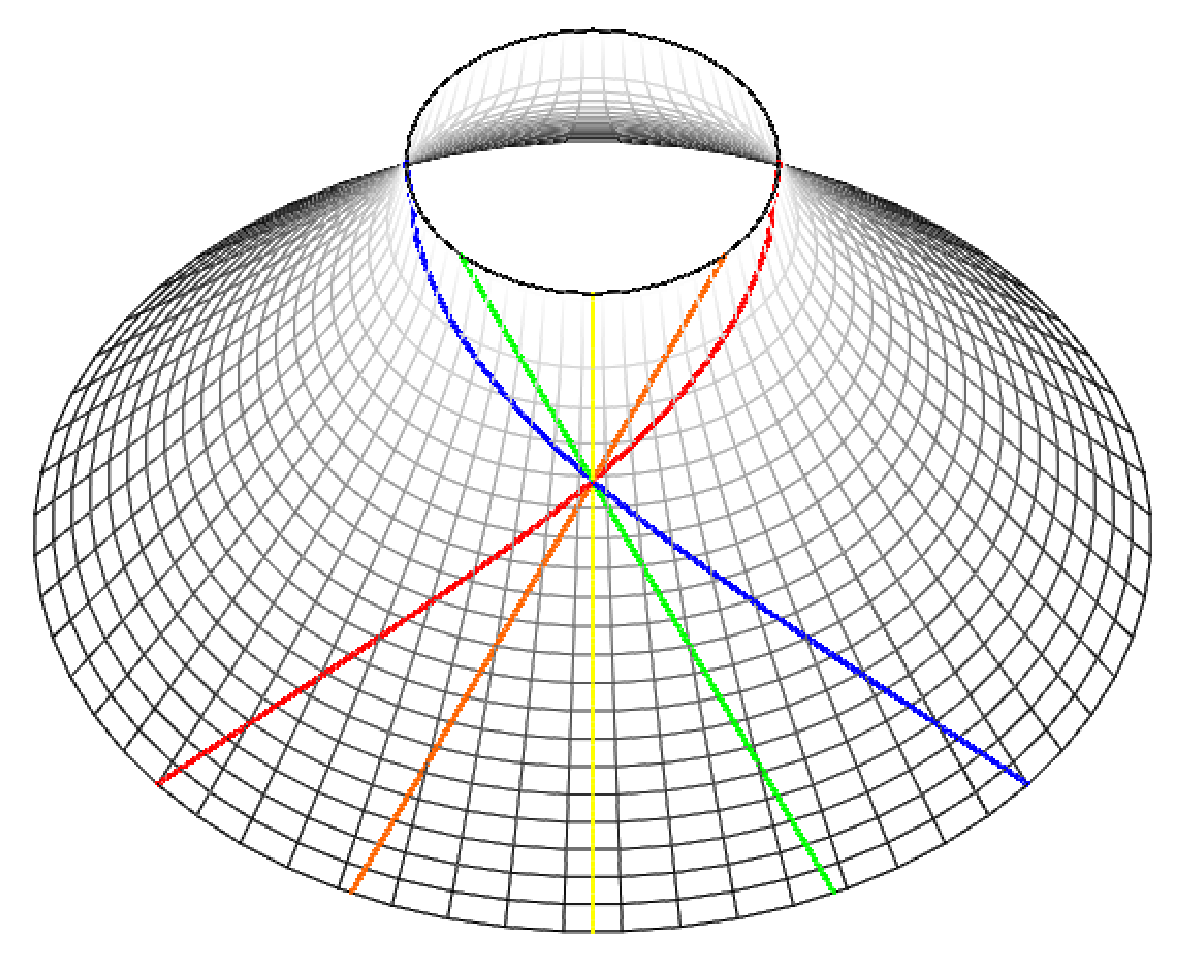
\includegraphics[height=3.25in]{dS_comoving_univ_rest.eps}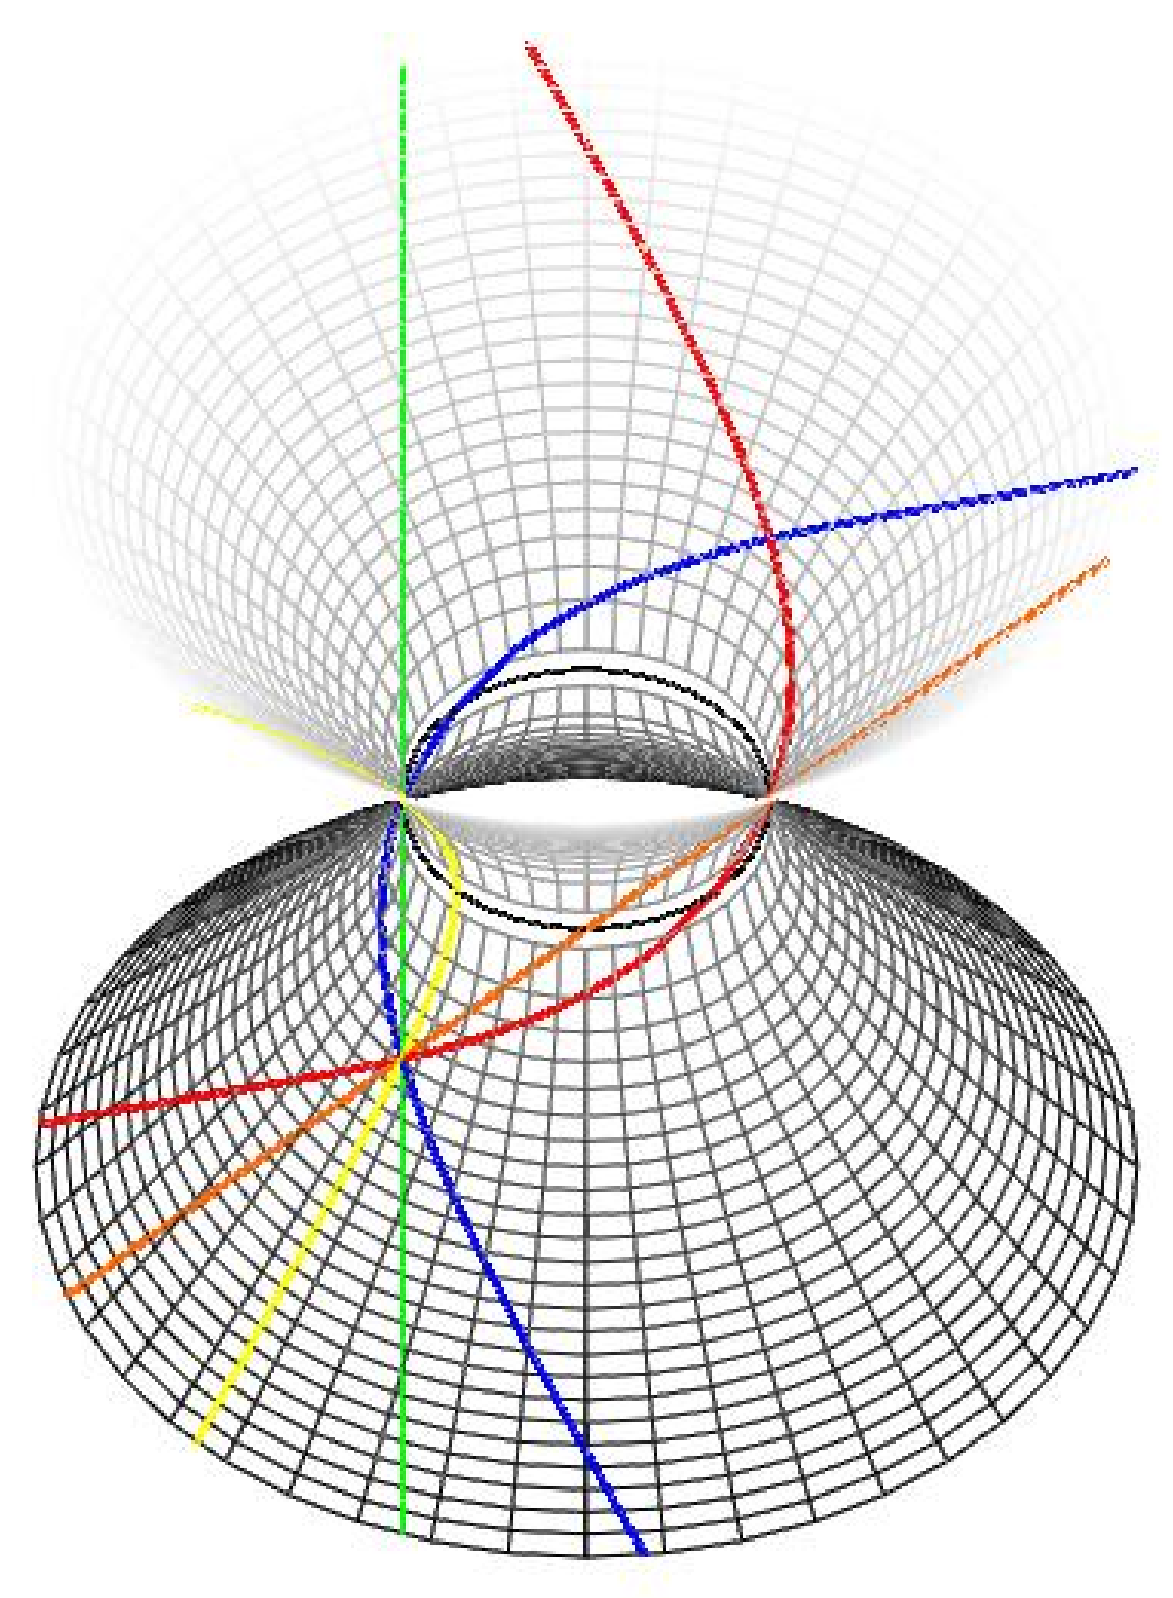
\includegraphics[height=3.25in]{dS_comoving_univ_null_extended.eps}}
\caption[The important worldlines of our closed, comoving de~Sitter cosmology, drawn on the de~Sitter 2-sphere in $\mathbb{M}^3$.]{The important worldlines of our closed, comoving de~Sitter cosmology, drawn on the de~Sitter 2-sphere in $\mathbb{M}^3$, with $t$ increasing downwards. The orange and green worldlines are straight null-lines which extend in either direction along the hyperboloid (doubly-ruled surface), and are therefore representative of particles that would be `at rest' in distinct cosmic rest-frames. The other three lines, with zero velocity through the 3-sphere (yellow) or twice that of a particle moving along a null-line (red and blue), represent possible paths attributed to photons; e.g., according to a particle moving along the green worldline, the yellow and blue lines represent the paths of photons that move radially inwards and outwards, respectively.}\label{fig: dS_comoving_univ}
\end{figure}

A point which has to be considered before an adequate response can be made to this objection, which the line-elements we've previously considered actually attest to, is that in any `radially' symmetric pseudo-Riemannian line-element which centres about a particle's spatial position, positive values of the `radial' coordinate used to describe `outer space' actually truncate at the particle, and therefore cover only half of the spacelike slice of the de~Sitter sphere that the line-element describes,\footnote{Namely, half of the spacelike slice through which the coordinate transformation, say from the Cartesian embedding of the real Riemannian sphere in Minkowski space, remains valid;---where it is not imaginary.} while negative values of the `radius' describe the particle's respective `inner space'. Therefore, from the perspective of all `massive particles', `photons' travelling along comoving geodesics of the cosmic void, must be those which move in the negative `radial' direction in the `radially' symmetric spacetime defined in Eq.~(\ref{sphersymm_t}), while those moving at twice the null rate in the same direction as the massive particle are `radially' outgoing; so, from the perspective of any massive particle---which we now define as one moving in any random direction, $\vartheta$, through the universe, with any velocity other than $d\vartheta/dt=0,\pm2(d\vartheta/dt)_{\mathrm{null}}$ (which correspond, due to general covariance, to massless particles travelling along null-lines in \textit{its} proper line-element, whether it is inertial ($d\vartheta/dt=const.$) or not)---another particle that moves through the universe in the opposite direction would be `moving radially inward through space faster than a photon'. Particles on oppositely directed orbits are therefore very different species.

But what is really meant by `oppositely directed orbits through the evolving 3-sphere'? In the two-dimensional representation given in Fig.~\ref{fig: dS_comoving_univ}, which graphs the cosmic evolution of a 1-sphere, this is quite easy to see, since there are two objectively well-defined directions around a circle; but it is not so clear as we come to consider the timelike evolution of a 3-sphere. For example, in the case of a 2-sphere it is possible to parallel transport a tangent vector along a path that would bring it back to the same point with the opposite (or any other) sense.\footnote{For example, transport a tangent vector $180^{\circ}$ along the great circle in the direction that it is pointing, and then $180^{\circ}$ along a perpendicular one, so that it arrives back at its original position with opposite sense.} In fact, the 2-sphere is not parallelisable, according to the hairy ball theorem \cite{Milnor1978}, so `directions of motion' on it can't be completely well-defined. It is therefore remarkable that the 3-sphere is parallelisable, as a 2-sphere worth of 1-spheres with a twist in the manifold \cite{Christian2011}, so that two universal `opposite directions of motion' can always be defined, as with the evloving 1-sphere depicted in Fig.~\ref{fig: dS_comoving_univ}. 

So, further to the assumption that the cosmographical line-element should be parametrised by the evolution of massive particles travelling along null-lines on the de~Sitter sphere, so that the paths of massless particles satisfying $d\vartheta/dt=0$, which actually move relative to a rest-frame observer at the same rate that the observer moves through the universe, can therefore be \textit{defined} as null in the corresponding spacetime geometry, we recognise that the direction of motion of these fundamental worldlines can be defined by any inertial particle according to a universal parallelisation.

And the gist of the idea, as it seems to apply according to the discussion in \S~\ref{sec_DPM}, is that an inertial particle's velocity through the 3-sphere should be able to be related, in the local radially symmetric coordinate frame, to some sort of \textit{radial} momentum, even though those coordinates describe the particle as remaining at the origin---and the two `opposite directions of motion' that we are now considering, are therefore opposite `radial' directions of motion (i.e., relative `inwards' and `outwards', corresponding to positive or negative radial velocity), which is not described as taking place \textit{along} the radial coordinate in the proper frame of such a particle (i.e., a particle does not describe itself as `expanding' or `contracting'), but is still described by the metric, Eq.~(\ref{sphersymm_t}), in a different way, because such particles are actually moving through the real dynamic universe along inertial paths which are not geodesics. 

What seems to be an interesting consequence of the fact that there are three distinct velocities for photons, is that the mass of any particle is not a single value, but a triplet---an objectively well-defined superposition of three values, which seems to indicate a basic relation between our theory of relativity and something like de~Broglie-Bohm theory---and the physical difference we shall find, between particles that do move with opposite velocities through the universe, is that their masses should therefore be each other's negatives. 

But because we are primarily concerned with describing the cosmic evolution from the perspective of a collection of `positive' mass particles, we can begin by considering the motion of all particles through the universe as being all with the same sense of direction, corresponding to one set of null-lines on the de~Sitter sphere. When this is done, it is actually quite simple to sort out the most general form for the line-element, even without using a coordinate transformation from any standard de~Sitter line-element, since Eddington's symmetry idea applies similarly in this case; viz., we take the homogeneous three-dimensional universe to be moving `radially' outwards in the cosmic time dimension, but re-define one spatial coordinate to meet the requirement, that a \textit{photon} moving in either direction in that dimension, follows a null-line---i.e.,
\begin{equation}
ds^2=-B(r_\mathrm{SdS}},t_\mathrm{SdS}})dr_\mathrm{SdS}}^2+A(r_\mathrm{SdS}},t_\mathrm{SdS}}) dt_\mathrm{SdS}}^2+r_\mathrm{SdS}}^2\left(d\theta^2+\sin^2\theta{d\phi^2}\right).\label{sphersymm_r}
\end{equation}
We have thus performed a speed-time contraction on the de~Sitter sphere \cite{Bacry1968} which preserves the metrical description of the flow of cosmic time that is given in the comoving coordinates of Eq.~(\ref{dS_comoving_univ}); but rather than describing space according to the inertial geodesics of that universe, and preserving the basic null-structure of the void, the spatial coordinates are described according to the null worldlines that all move in the same direction with respect to a parallelisation of the universe, relative to which the (unaccelerated) inertial \textit{geodesics} really do move at the cosmic null rate, so that they may reasonably be defined as null lines in the contracted line-element. The result of solving the vacuum Einstein equation for this general line-element has a well-known form, similar to the solution when $A$ and $B$ have the opposite signs, as in Eq.~(\ref{sphersymm_t}); in addition to those due to its `radial' symmetry, the metric may also be given with a $t_\mathrm{SdS}}$-like Killing vector, so that a particle's velocity through space does not depend on position; and the inhomogeneity in the spatial coordinate $t_\mathrm{SdS}}$ merely reflects the inversion of perspective that has been written into the line-element, according to which that spatial coordinate should now run parallel to the oppositely-directed null-lines of the real de~Sitter void. 

In the following chapter, we will analyse the cosmology entirely from this inverted perspective, beginning from a derivation of the SdS geometry, as the simple solution to the vacuum Einstein equation, from this perspective, that describes the cosmic evolution of this universe along $r_{\mathrm{SdS}}$. And it will eventually be shown, that from this perspective the universe would be perceived as a massive one that began from a singularity at $r_\mathrm{SdS}}=0$, in such a manner that, from the cosmic rest-frame, space would be perceived as being flat, with the universe expanding from this finite beginning, and scaling according to $r_\mathrm{SdS}}(\tau)\propto\sinh^{2/3}\left(\frac{3}{2}\sqrt{\frac{\Lambda}{3}}\tau\right)$---the precise scale-factor of the flat $\Lambda$CDM model.